\chapter{Impedance Transformation in a lossless medium using a Smith Chart}\label{lec:lec8}
\section{Objectives}

\begin{enumerate}[(i)]
\item How to develop the Voltage Standing Wave Ratio(VSWR) set of circles.
\item Relationship between impedance and admittance.
\item How to determine reflection coefficient graphically.
\item How to determine impedance transformation graphically.
\item How to locate maximum and minimum voltage, and current points on the transmission line on the smith chart.
\end{enumerate}
Previously, we developed a graphical tool by transforming the complex impedance of a transmission line into the gamma plane called the smith chart. This was a superposition of constant resistance circles on constant reactance circles lying within the limit circle $|\Gamma| \leq 1$. Before we go into the use of the SMITH CHART for transmission line calculations, we develop one more set of circles called the constant VSWR circles and then superpose it in the smith chart.\\\\ We know that:
\begin{equation*}
\Gamma(l) =\Gamma_L e^{-j2\beta{l}}
\end{equation*}
where l = distance from load point towards generator.\\
$\Gamma_{L}$ = voltage reflection coefficient at load end.\\ 	
$\beta$\ = phase constant of the transmission line.\\\\
\textbf{NOTE:}	We are still discussing lossless transmission lines for which the attenuation constant is zero.
\begin{equation*}
\Gamma{(l)}=|\Gamma_{L}|e^{j\theta_L}.e^{-j2\beta l}
\end{equation*}
where	$\theta_L$ = phase angle of deflection of the load.
\begin{equation}
\Gamma{(l)} =|\Gamma_L|e^{j(\theta_L - 2\beta{l})}
\end{equation}
That is, total phase = $\theta_L - 2\beta{l}$.\\
Hence the reflection coefficient $\Gamma{(l)}$ has magnitude $|\Gamma_L|$ on the complex gamma plane but it's phase angle varies with distance from the load end. Since $l$ is positive when moving towards the generator, therefore, the phase increases in negativity. The distance of the point $|\Gamma_L|$ from the centre of the circle remains constant but it's angle changes with a change in $l$. Hence $|\Gamma_L|e^{j(\theta_L - 2\beta l)}$ represents a constant VSWR circle having the same centre of origin with that of the complex gamma plane.

When moving towards the generator with increasing length, $l$, a corresponding anti-clockwise rotation in the gamma plane is experienced. On this circle, the magnitude of the reflection coefficient is the same no matter what point we are, but the angle differs and we know that:
\begin{equation}
VSWR = \frac{1 + |\Gamma_L|}{1 - |\Gamma_L|}
\end{equation}
\begin{figure}[h]
\centering
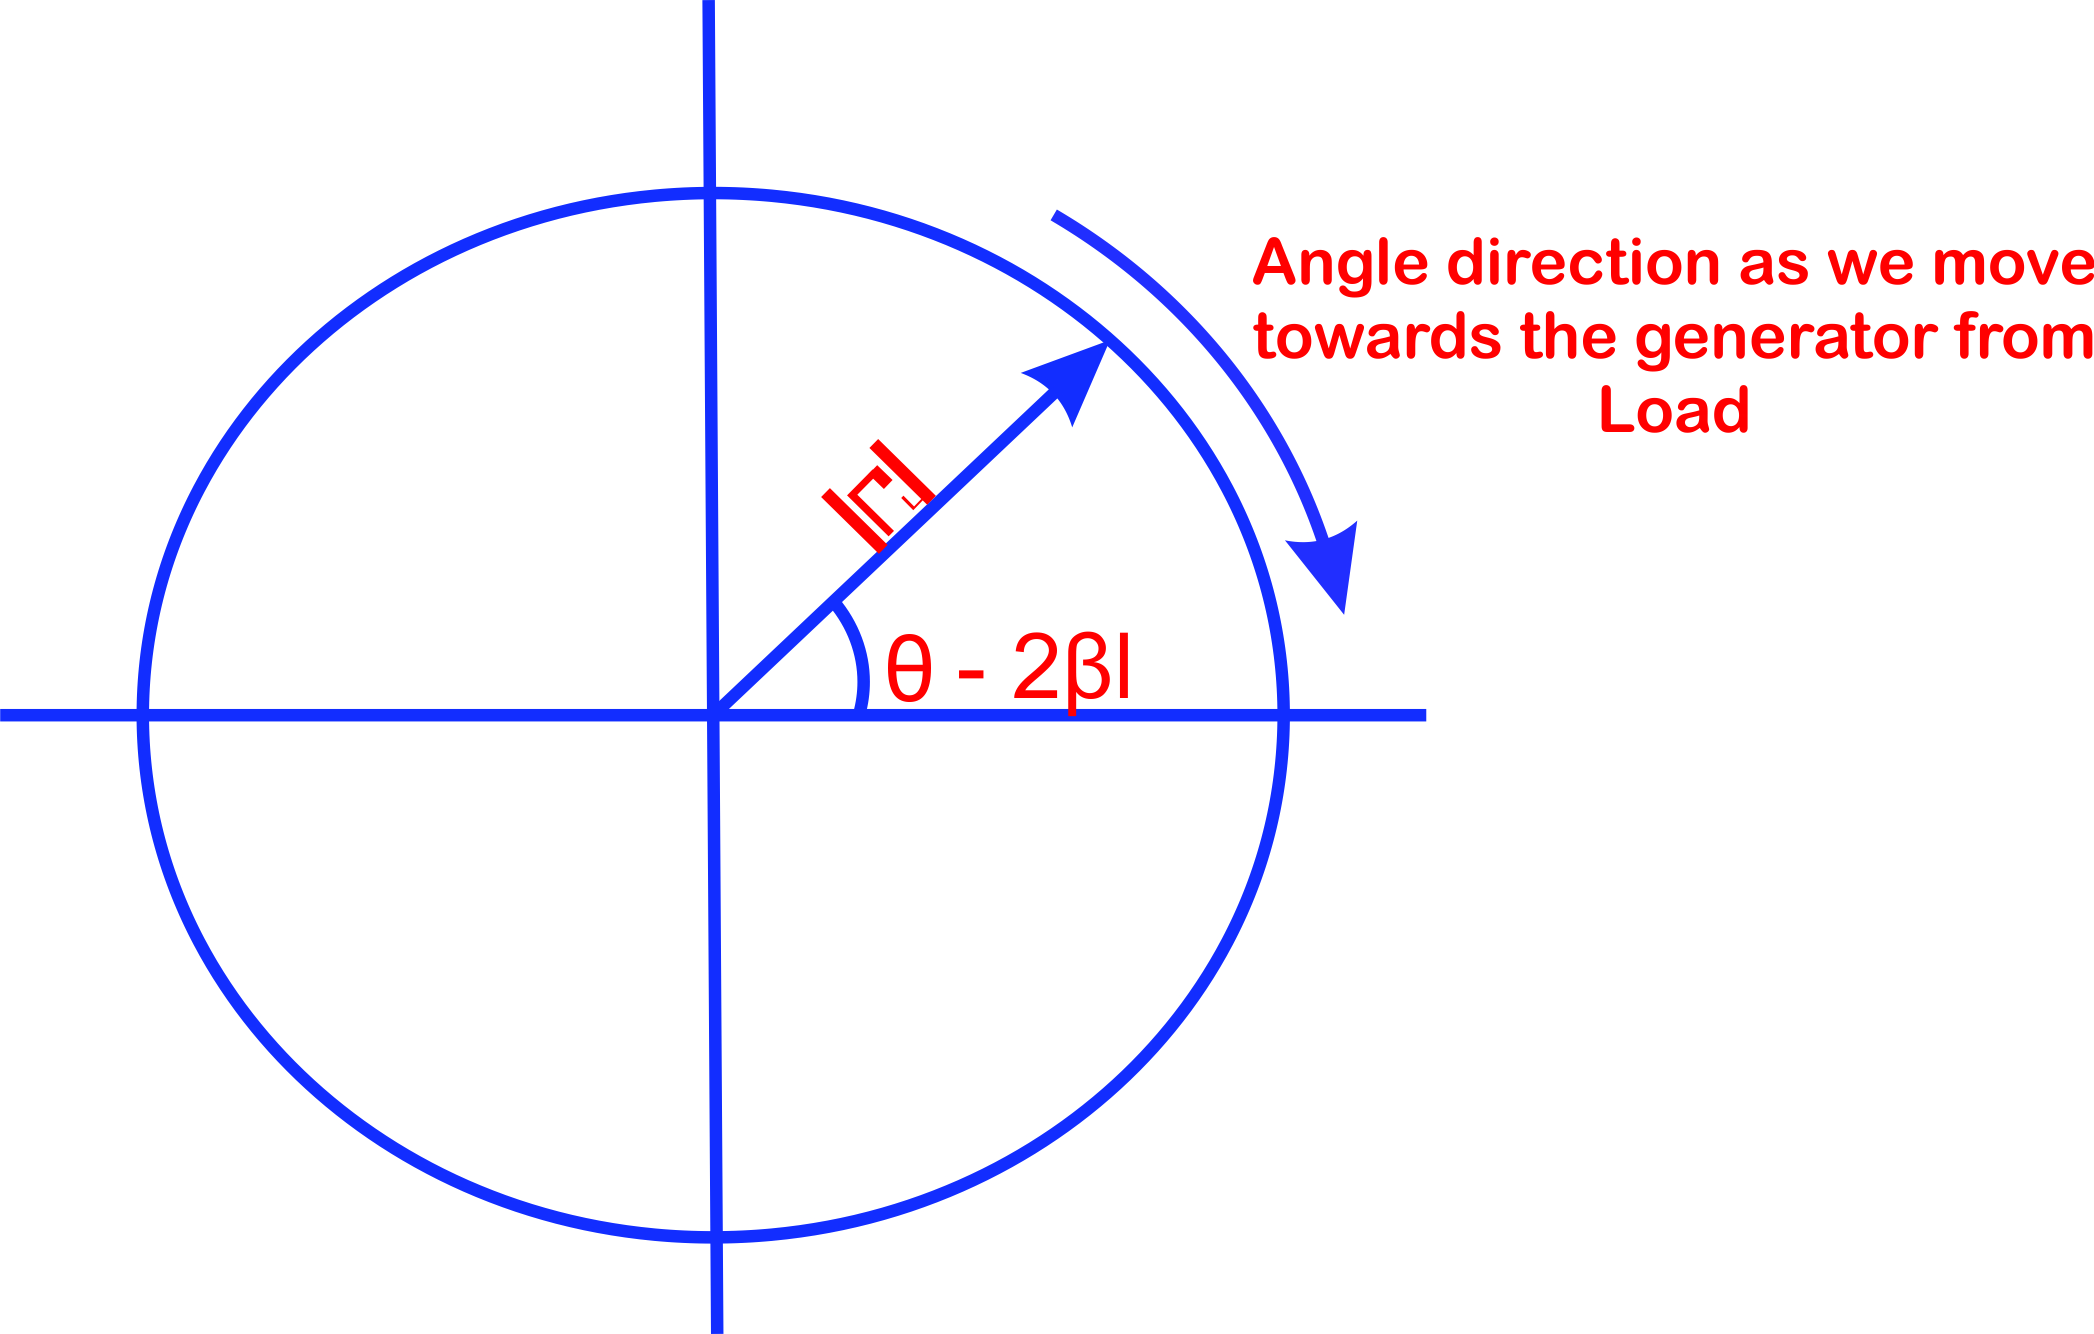
\includegraphics[width=0.7\linewidth]{./graphics/lkjhgryn}
\caption{Constant VSWR Circle}
\label{fig:lkjhgryn}
\end{figure}

Since $|\Gamma_L|$ is same at any point on the circle, then the VSWR is same for all points on the circle, hence we call the circle a constant VSWR circle. Note that while solving transmission line problems, we have to draw circles of constant VSWR circles on the smith chart so the smith chart readily gives the constant resistance and reactance circles in the limit circle of $|\Gamma_L|\leq 1$.
\begin{figure}[h]
\centering
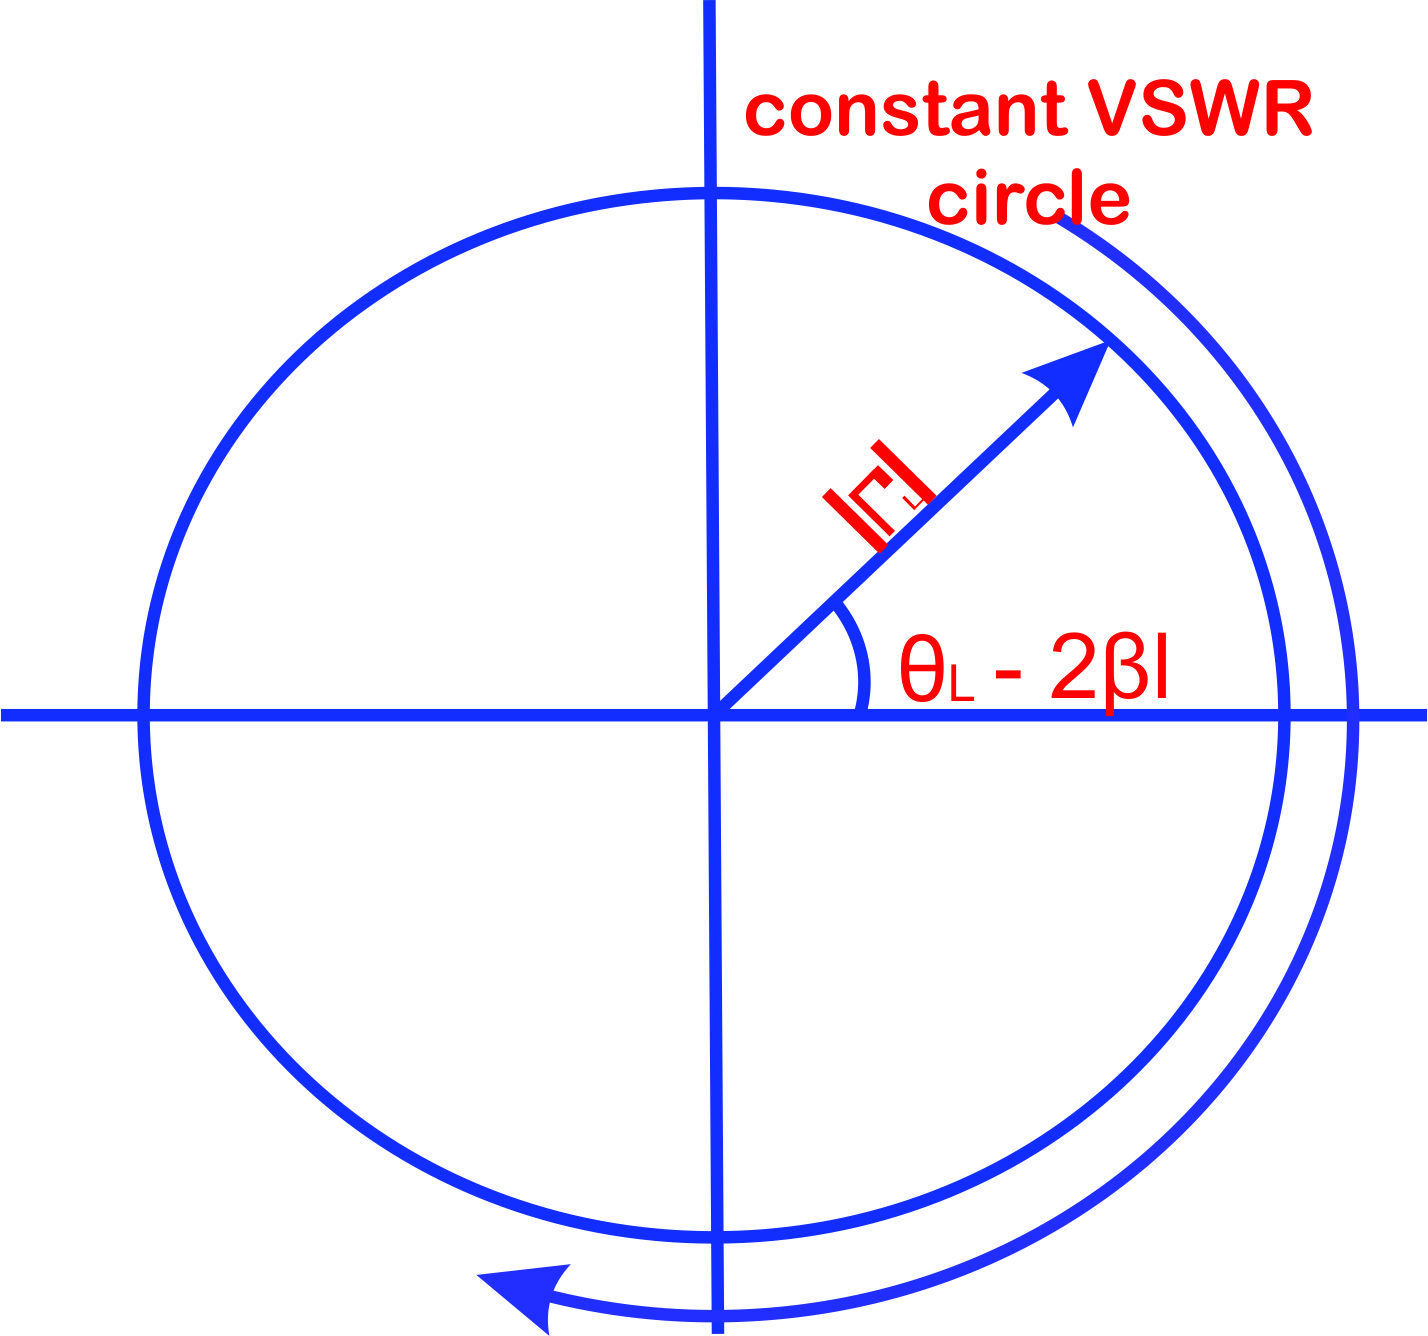
\includegraphics[width=0.5\linewidth]{./graphics/qwertyhgf}
\caption{Constant VSWR Circle}
\label{fig:qwertyhgf}
\end{figure}

One should always note that the centre of all VSWR circles is same as that of the origin of  the complex gamma plane for all passive loads. Therefore, the magitude of the reflection coefficient is always less or equal to 1. So the VSWR circles are centred at the origin of the gamma plane and maximum $|\Gamma_L|=1$. Larger radius of $|\Gamma_L|$ gives more reflection coefficient with lower impedance match and smaller radius of  $|\Gamma_L|$ gives smaller magnitude of reflection coefficient and a better impedance match.

When we have impedance matching on the smith chart, visually speaking, we can say that the point closest to the centre of the smith chart is better for impedance matching because it represents a smaller magnitude of reflection coefficient. With the understanding of superimposing the constant VSWR circle on the smith chart, we can therefore solve the transmission line problem.
\begin{figure}[h]
\centering
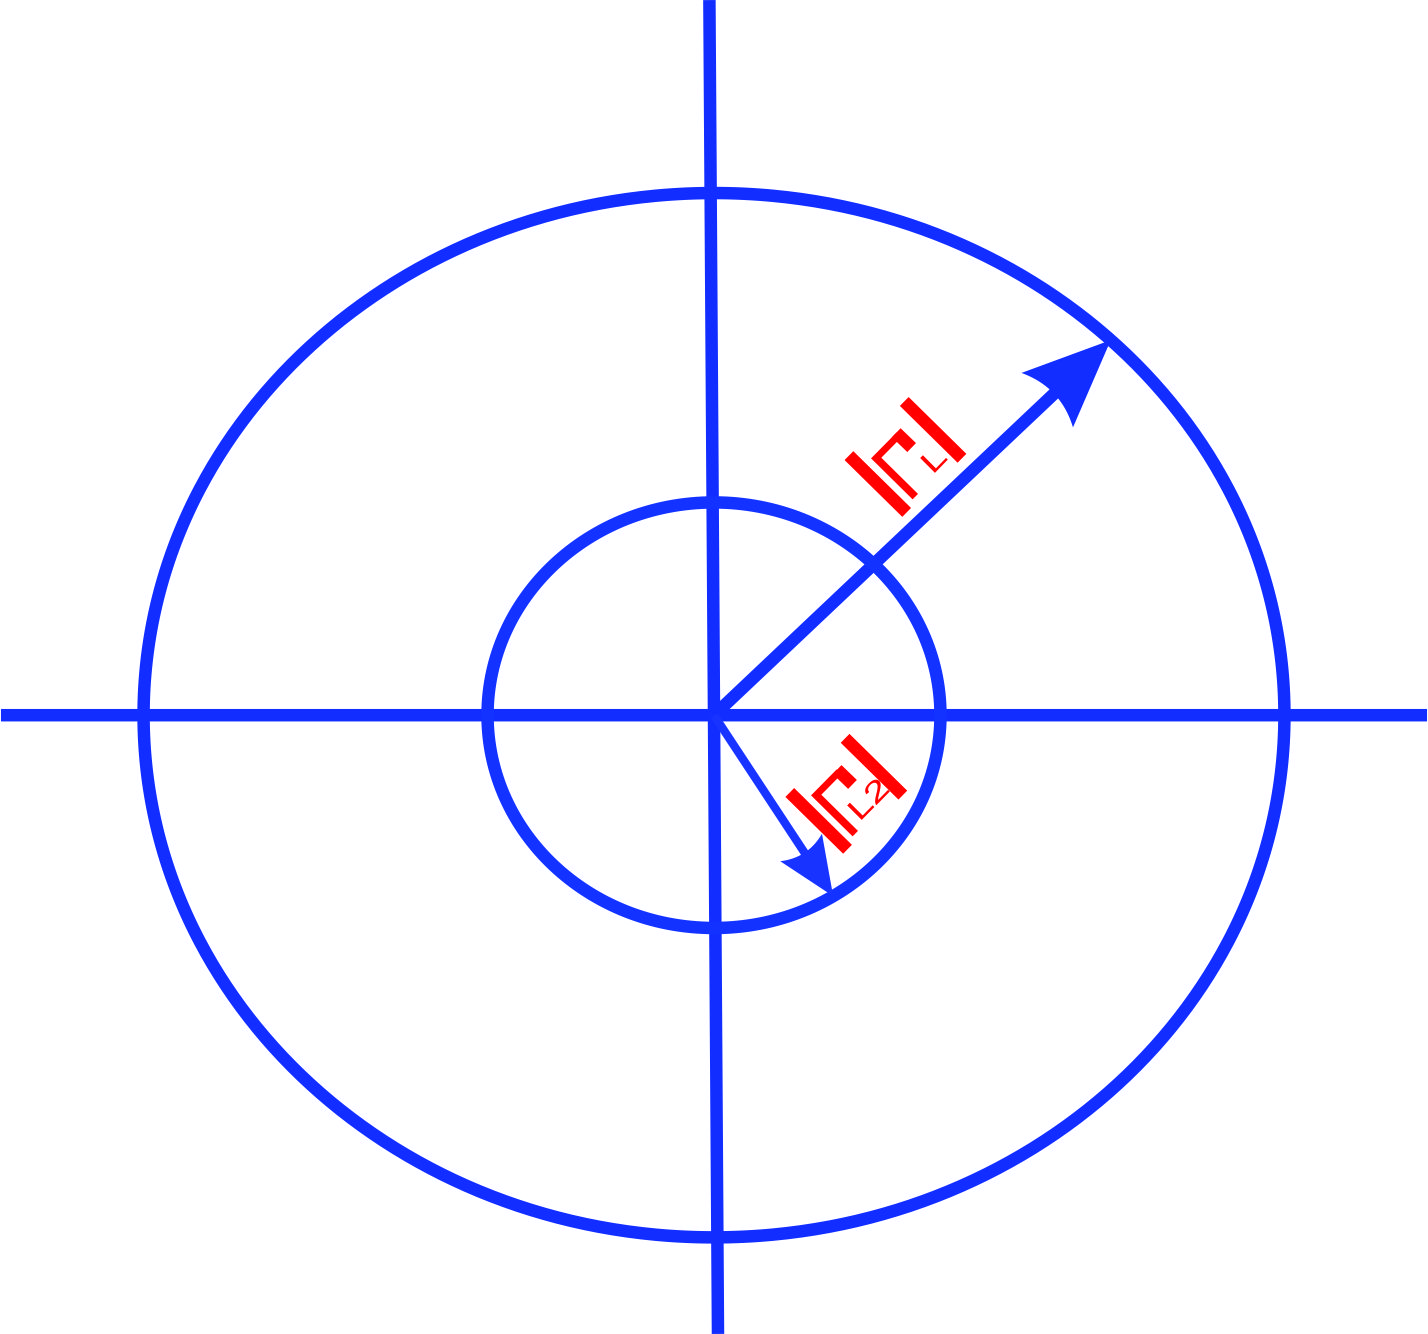
\includegraphics[width=0.57\linewidth]{./graphics/poiuyfd}
\caption{Impedance match with less reflection}
\label{fig:poiuyfd}
\end{figure}

However as we have said, you may have connections in transmission lines which are in the form of parallel connections and we know that from circuit analysis, anywhere we have parallel connections, it is easier to deal with admittances rather than impedances. Before now, we have been discussing load impedances and load characteristics impedance of transmission lines. However, if we have to make parallel connections on the transmission line, we represent the load as admittances and characteristics admittance before we carry out the analysis on the smith chart. We can therefore determine how the smith chart will work if we do all calculations in terms of admittances. Since the smith chart gives the normalized impedances of the transmission line, the same thing will be derived for admittances so we shall first define the normalized admittance of the transmission line and from that, we would require what is called the characteristic admittance of the line. First we define the characteristic admittance.
\section{Admittance}
\begin{equation}
Y_o= \frac{1}{Z_o}
\end{equation}
Then, every admittance is normalized to this,
\begin{equation*}
\overline{Y} = \frac{Y}{Y_o} 
\end{equation*}
\begin{equation*}
\space  \overline{Y}_L = \frac{Y_L}{Y_o}
\end{equation*}
Recall from previous chapters:
\begin{equation*}
\Gamma = \frac{Z-Z_o}{Z+Z_o} 
\end{equation*}
The impedance Z is then expressed as the inverse of admittance $\frac{1}{Y}$. When we normalize all admittances with respect to the characteristics admittance, we can then imply that the reflection coefficient in terms of the admittance can be expressed as:
\begin{equation*}
\Gamma = \frac{\frac{1}{Y} - \frac{1}{Y_o}}{\frac{1}{Y} + \frac{1}{Y_o}}
\end{equation*}
Then, the equation is simplified to give:
\begin{equation}
\Gamma= \frac{Y_o - Y}{Y_o + Y} 
\end{equation}
Dividing the numerator and denominator by $Y_o$:
\begin{equation*}
\Gamma= \frac{1 - \frac{Y}{Y_o}}{1 + \frac{Y}{Y_o}}
\end{equation*}
The final equation is given as:
\begin{equation*}
\Gamma= \frac{1 - \overline{Y}}{1 + \overline{Y}} = -1 (\frac{\overline{Y} - 1}{\overline{Y} + 1}) 
\end{equation*}
The negative sign indicates a phase change making reflection coefficient equal to:
\begin{equation}
\Gamma = \frac{\overline{Y} - 1}{\overline{Y} + 1}e^{j\pi}
\end{equation}
As -1 is a phase change of $\pi, e^{j\pi} = cos\pi + jsin\pi = -1$\\\\
So the reflection coefficient written in terms of normalized admittances is same as reflection coefficient written in terms of normalized impedance except for the 180$^o$ phase change brought in by $e^{j\pi}$.\\
This implies that same value is derived for reflection coefficient when calculated using the normalized impedance or admittance but for a phase shift of 180$^o$ which would be experienced on the transmission line. In other words, on the complex gamma plane of the smith chart, the 180$^o$ phase shift will correspond to a rotation of 180$^o$. Essentially, the normalized impedance and admittance can be calculated in the same way except when we are doing calculations for normalized admittances then, there is a rotation of 180$^o$ on the complex gamma plane otherwise all other values and parameters remain unchanged.
\begin{figure}[h]
\centering
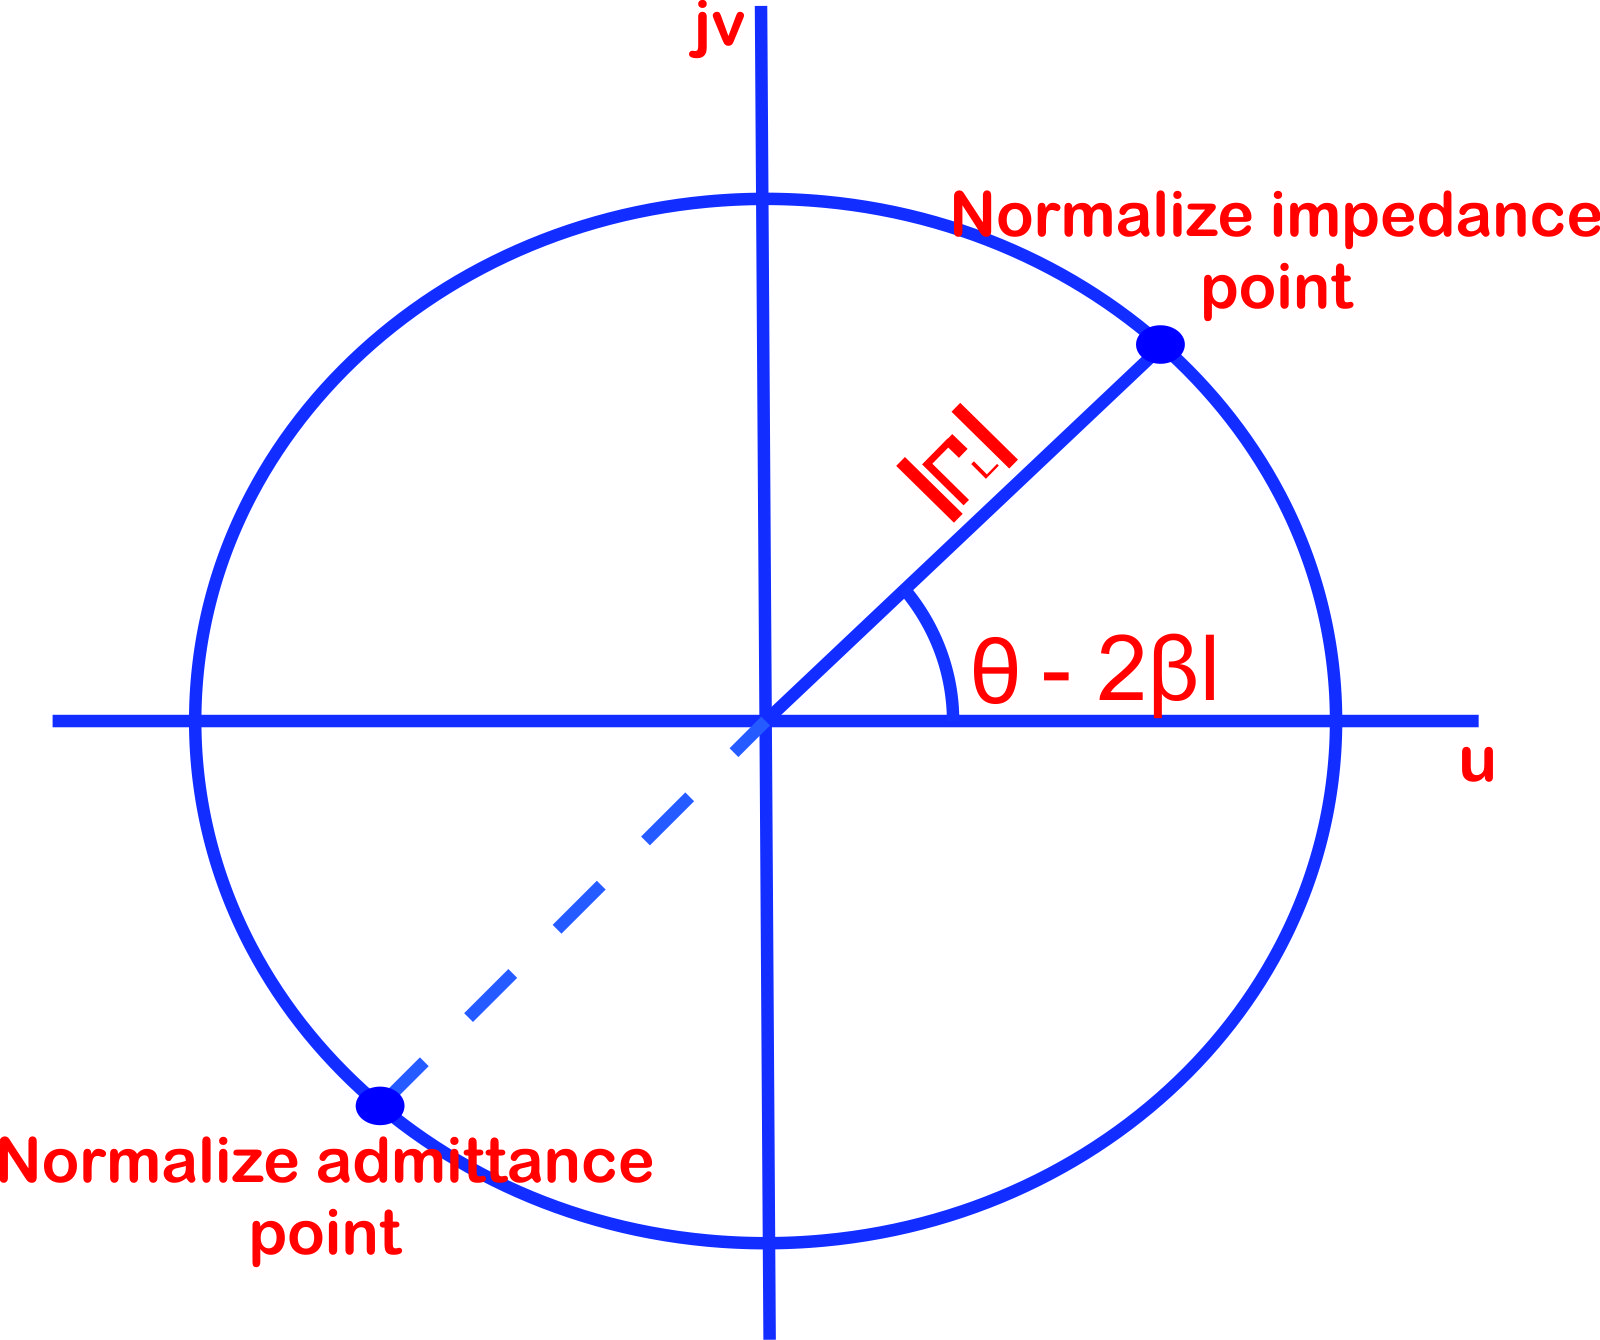
\includegraphics[width=0.6\linewidth]{./graphics/zstyuiou}
\caption{Normalized impedance point}
\label{fig:zstyuiou}
\end{figure}

Hence as far as the set of circles are concerned on the smith chart, any point on the smith chart rotated by 180$^o$ corresponds to a set of circles called the normalized admittance. Let's then say that:
\begin{equation*}
\overline{Y} = g + jb = conductance + j(susceptance.)
\end{equation*}
\begin{equation*}
\overline{Y}=\frac{G + jB}{Y_o} = g + jb
\end{equation*}
So if we have admittance on a line given by G + jB, and characteristics admittance $Y_o$, we can calculate the normalized admittance as 
\begin{equation*}
\overline{Y} = g + jb
\end{equation*}
If we interchange r with g and x with b, we can get a set of circles which will be \textbf{constant conductance circle and constant susceptance circle} which is similar to the constant resistance and reactance circles except that they are rotated by 180$^o$. Hence every point on our smith chart is flipped and so the clustered point goes to the left as shown in the figure below.

So nothing has changed as far as the smith chart is concerned unless that it is rotated by $180^o$. If we keep the axis of the complex reflection coefficient the same, then the smith chart is rotated by $180^o$. Alternatively, we keep the smith chart the same as the original, rotate the complex gamma axis by $180^o$ before doing calculations for admittances. So, if we develop an understanding that we will not rotate the smith chart, that means we want to use it in its original form, that is, the most clustered part of it to our right, then if we do the impedance calculations, the positive real axis is towards right and the positive imaginary axis goes up. However, during calculations using the smith chart unchanged for admittances, the positive real axis is towards the left and the  positive imaginary axis will be downwards. Normally, whenever we do the smith chart calculations, we do not rotate the smith chart. For the impedance, the gamma axis is the  positive top right plane and for admittances, the bottom left plane is the positive plane. Depending on whether we are doing calculations for the impedance or admittances and if we require fixed measurement in the complex gamma plane, then the axis has to be rotated appropriately by $180^o$ depending on whether we are using the impedance or admittance. However if we do not want to find the phase of the reflection coefficient, the axis of the gamma plane does not come into the picture but just the impedances and the admittance will do. So without worrying about the axis of the complex gamma plane, we can use the same Smith chart for the admittance as well as the impedance calculations. This is the reason why when you look at the Smith chart carefully, you will see that the upper half of the Smith chart is denoted by (x,b) and the lower part (-x,-b).The circles are denoted by either 'r' or 'g' so any normalized value of r is equal to the same normalized value of g as it will represent the same circle. So as long we are dealing with a normalized quantity, the impedance and admittance can be treated exactly the same way on the Smith chart. However, the normalized values of g and r or b and x have different meaning physically. Do they represent same physical conditions? The answer is NO!  For example r = 0 ; x = 0, corresponds to a short circuit condition, the impedance is zero at that point. However, if we take  a normalized value of admittance with g=0, b=0 which represents admittance equal to zero, it is not a short circuit but an open circuit condition on the line. Therefore, the normalized values of impedances and admittances can be  treated exactly the same way but when we go for the physical conditions, they are not treated as same. Let us therefore consider the points on Smith chart for the admittance with the special points replaced with b for r, g for x.
\begin{figure}[h]
\centering
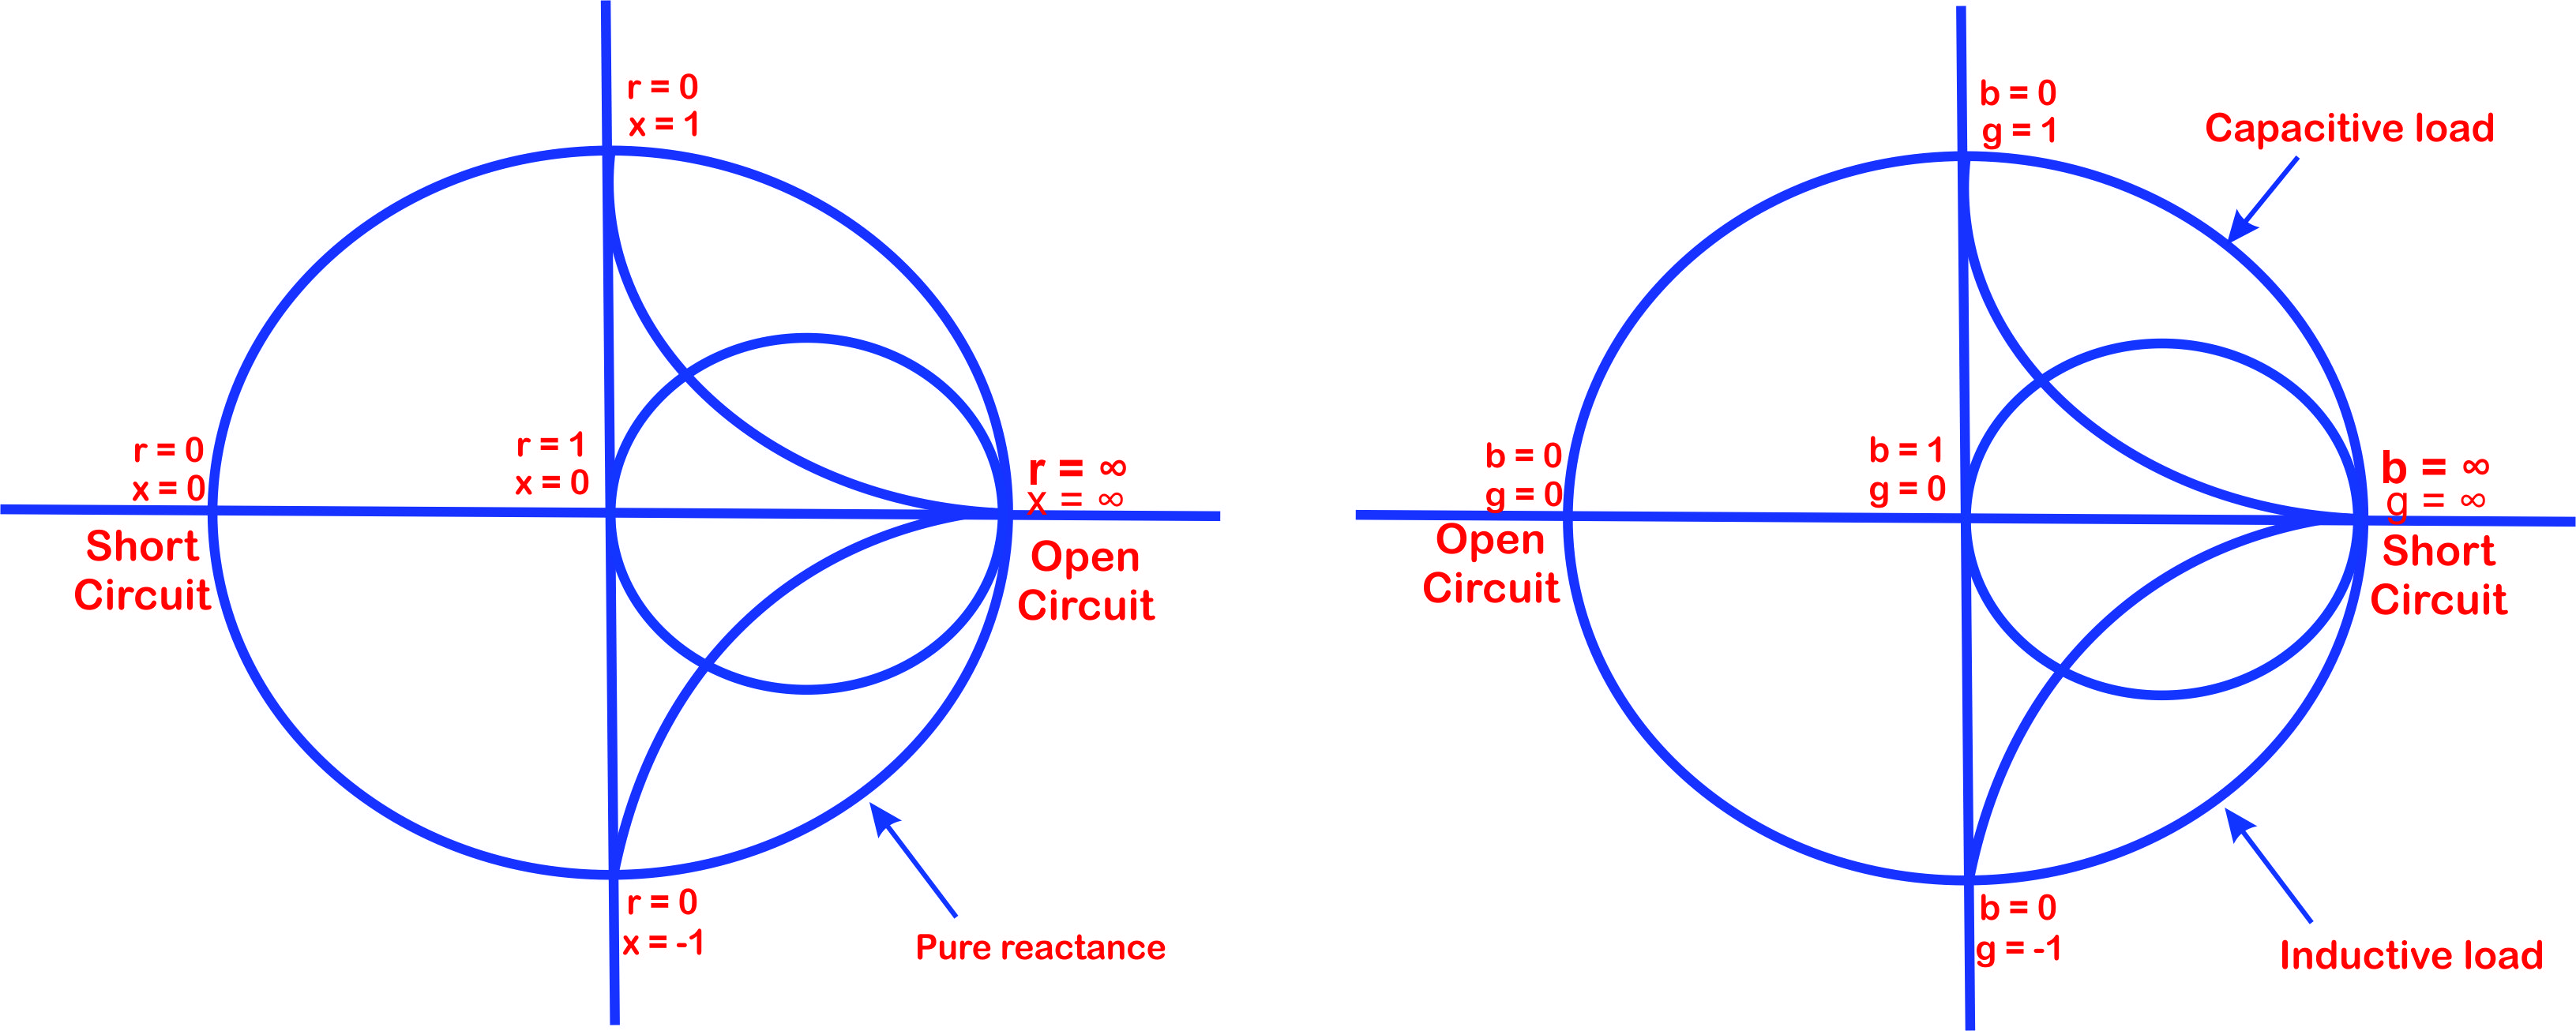
\includegraphics[width=1.0\linewidth]{./graphics/jnbkvfld}
\caption{Physical variation of impedance and admittance}
\label{fig:jnbkvfld}
\end{figure}

g = 0 b = 0 $\Longrightarrow$ open circuit and\\
g = $\infty$  b = $\infty$ $\Longrightarrow$  short circuit.\\
Keeping the Smith Chart fixed and doing the calculations with the admittances, the upper half of the Smith Chart represents capacitive loads and the lower half represents the inductive loads. With these in mind, the use of Smith chart for impedance or admittance calculation is very straight forward.\\
Now lets make use of the Smith chart to solve transmission line problems. 

\section{Use of Smith Chart for Transmission Line Calculation}
The simplest problem we can think of for transmission line is: For a given load, find the reflection coefficient at the load point. Analytically, we can use the formula $\frac{Z_L - Z_0}{Z_L + Z_0}$ but in using the Smith chart, the problem is much simpler to solve. Remember the impedance and admittance you have on Smith chart are all normalized quantities. So the first in any calculation on a Smith chart is to normalize all impedances and/or admittances with respect to characteristic impedance and/or characteristic admittance.

\subsection*{Procedure:}
\begin{enumerate}[(i)]
\item Normalize $Z_{L}$ to get $\frac{Z_{L}}{Z_{0}}$ = $\overline{Z}_{L}$ , read this point on the Smith chart, that is,  $r+jx$.
\item Identify the constant resistance and reactance circle with the value r and x respectively.
\item Determine the point of intersection of the r and x circles to give the reflection coefficient from which the length of the dotted line which gives $|\Gamma_L|$ and $\theta_L$ can be measured.
\begin{figure}[h]
\centering
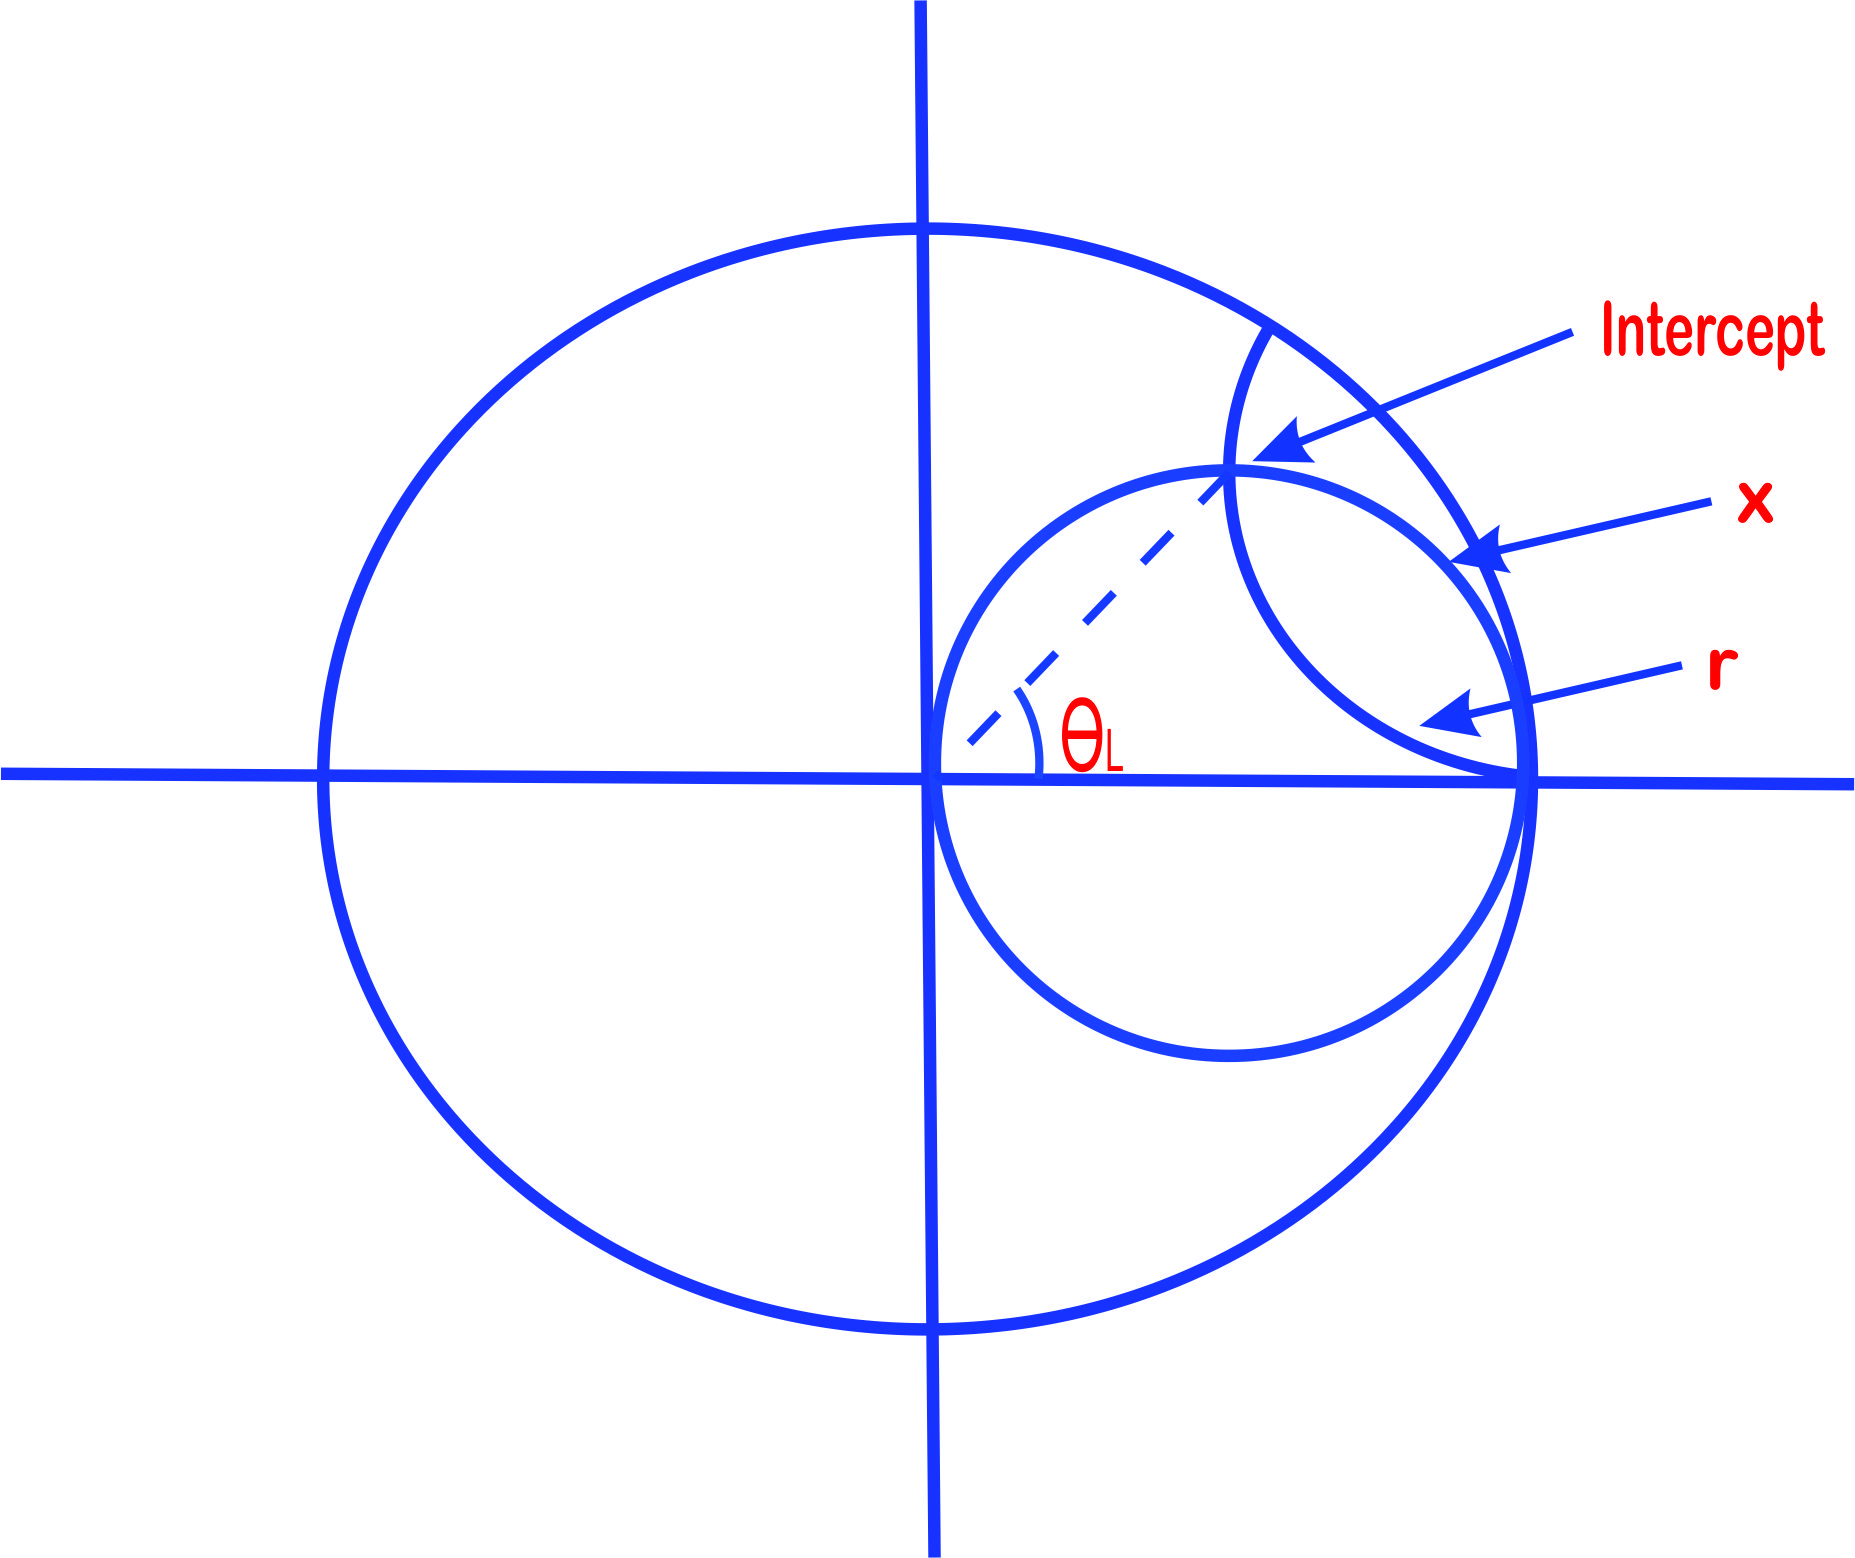
\includegraphics[width=0.6\linewidth]{./graphics/lfds}
\caption{Intercept Between Resistance and Reactance Circles}
\label{fig:lfds}
\end{figure}

So without doing any calculation, just by measuring its distance, and the angle, we get the magnitude of reflection coefficient   $|\Gamma_L|$
and phase angle $\theta_L$. Same thing we can do from the admittance perspective. Let $\overline{Y}$ = g + jb , we will see the intercept point on the Smith Chart for admittance too. However, to find out the complex reflection coefficient, recall the positive real axis is the one to the left for admittance since we have kept the Smith chart fixed. For admittances, the current axis has to be rotated by $180^o$. The distance from origin to that point gives you  $|\Gamma_L|$ but the phase measured from the  positive real axis shows $\theta_L$. 
\begin{figure}[h]
\centering
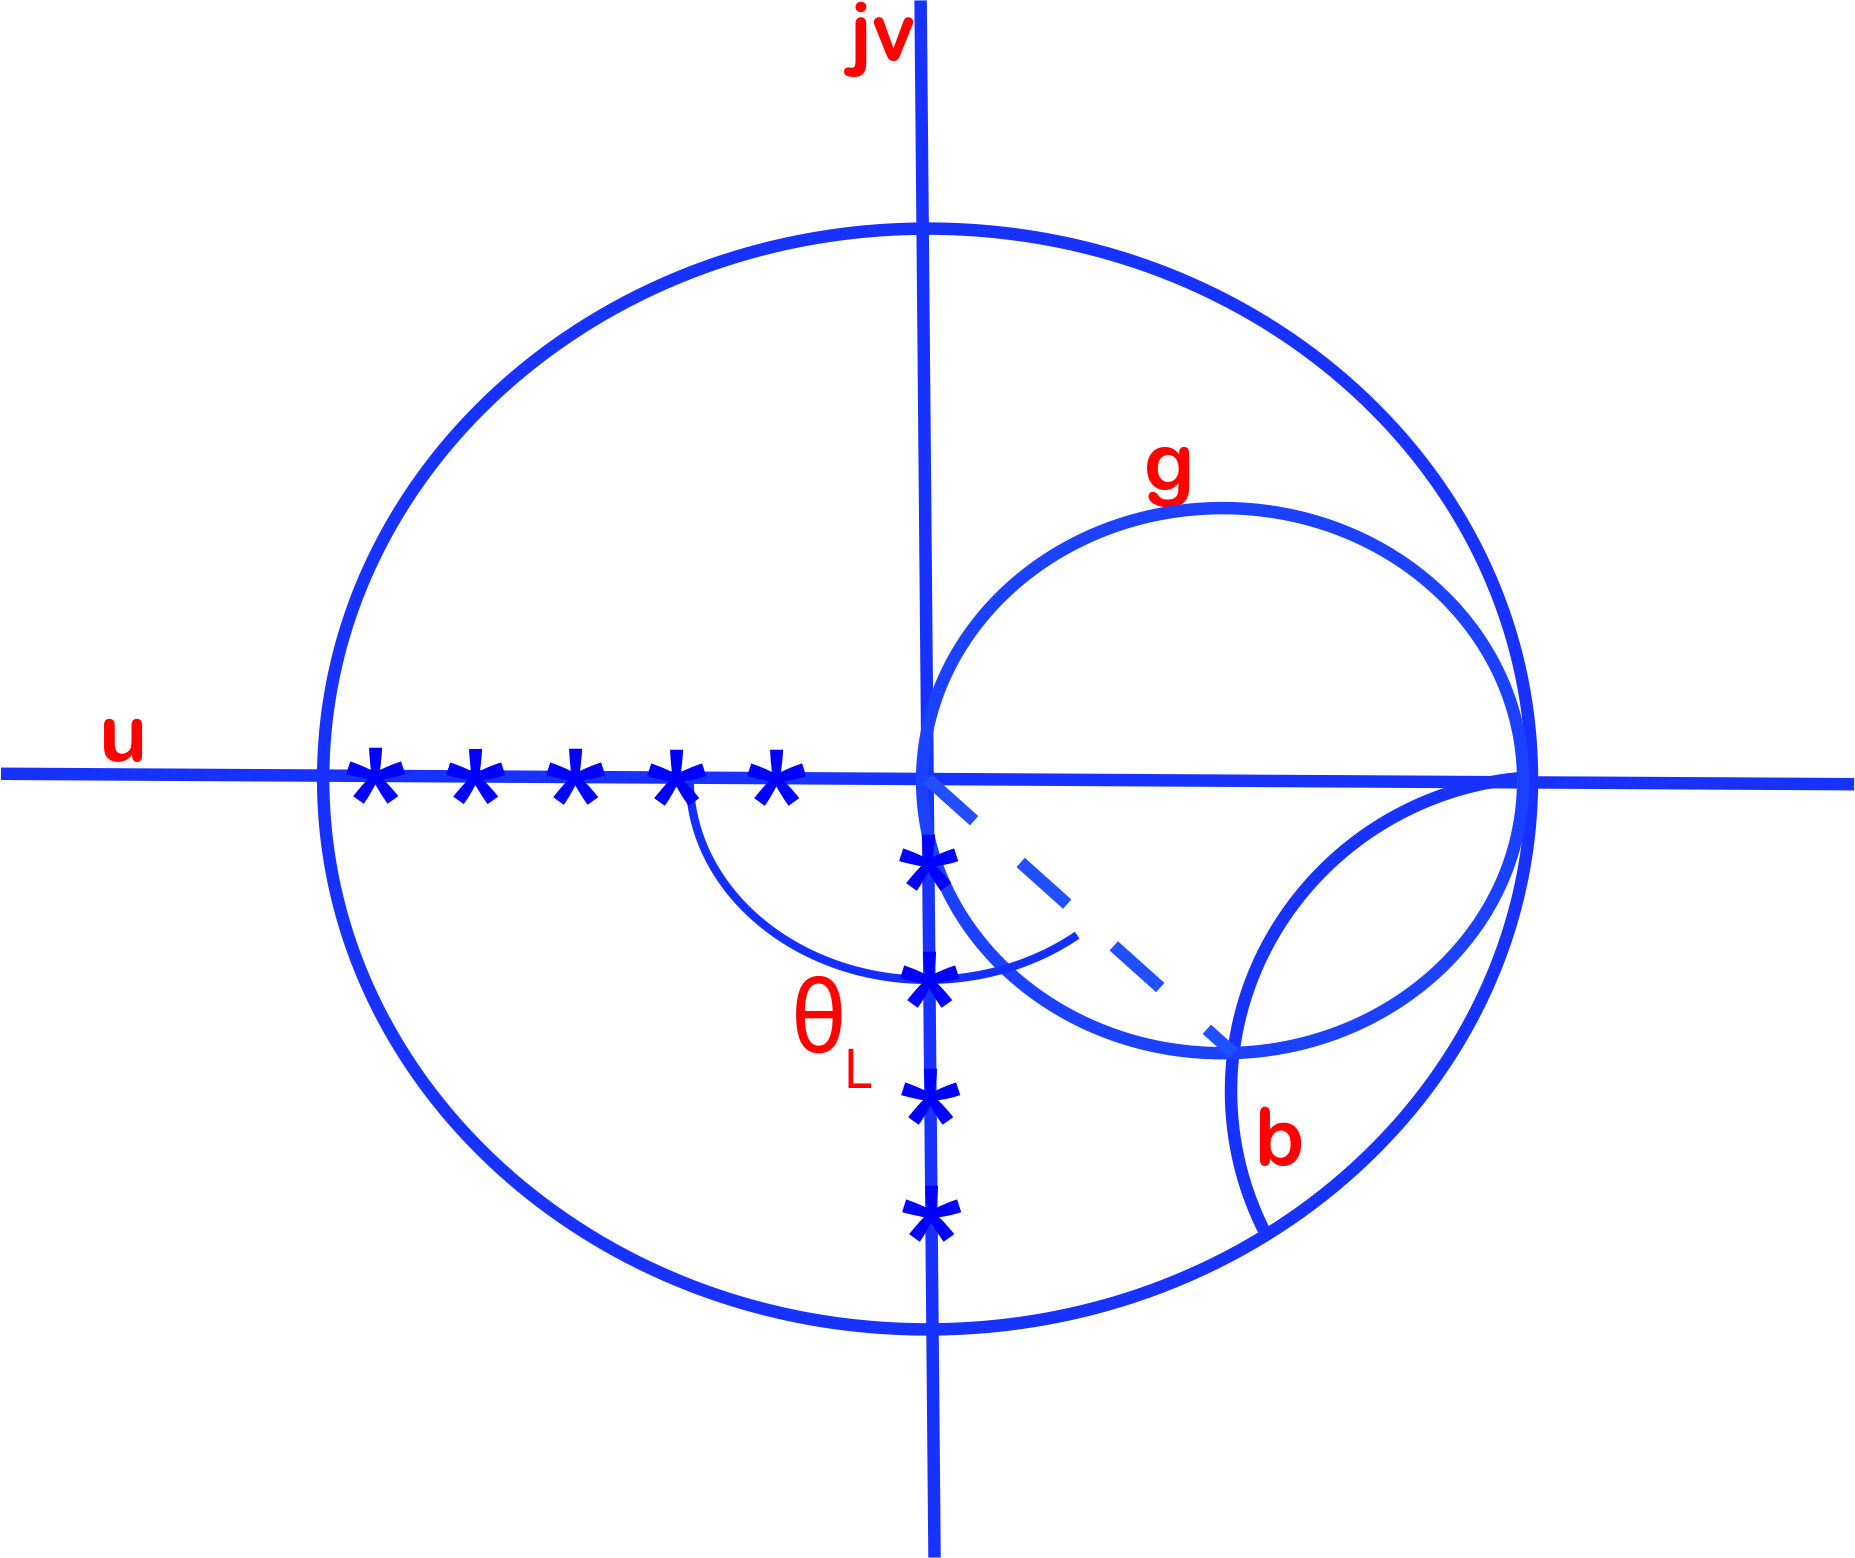
\includegraphics[width=0.6\linewidth]{./graphics/KJHGFDS}
\caption{Admittance Smith Chart at a $180^o$ phase shift}
\label{fig:kjhgfds}
\end{figure}
 
\subsection*{Procedure:}
\end{enumerate}


If the load impedance is given and we are asked to find the reflection coefficient and load impedance at another point $l$ on the transmission line, that is:

\section{Impedance transformation problems with the Smith Chart}
\begin{figure}[h]
\centering
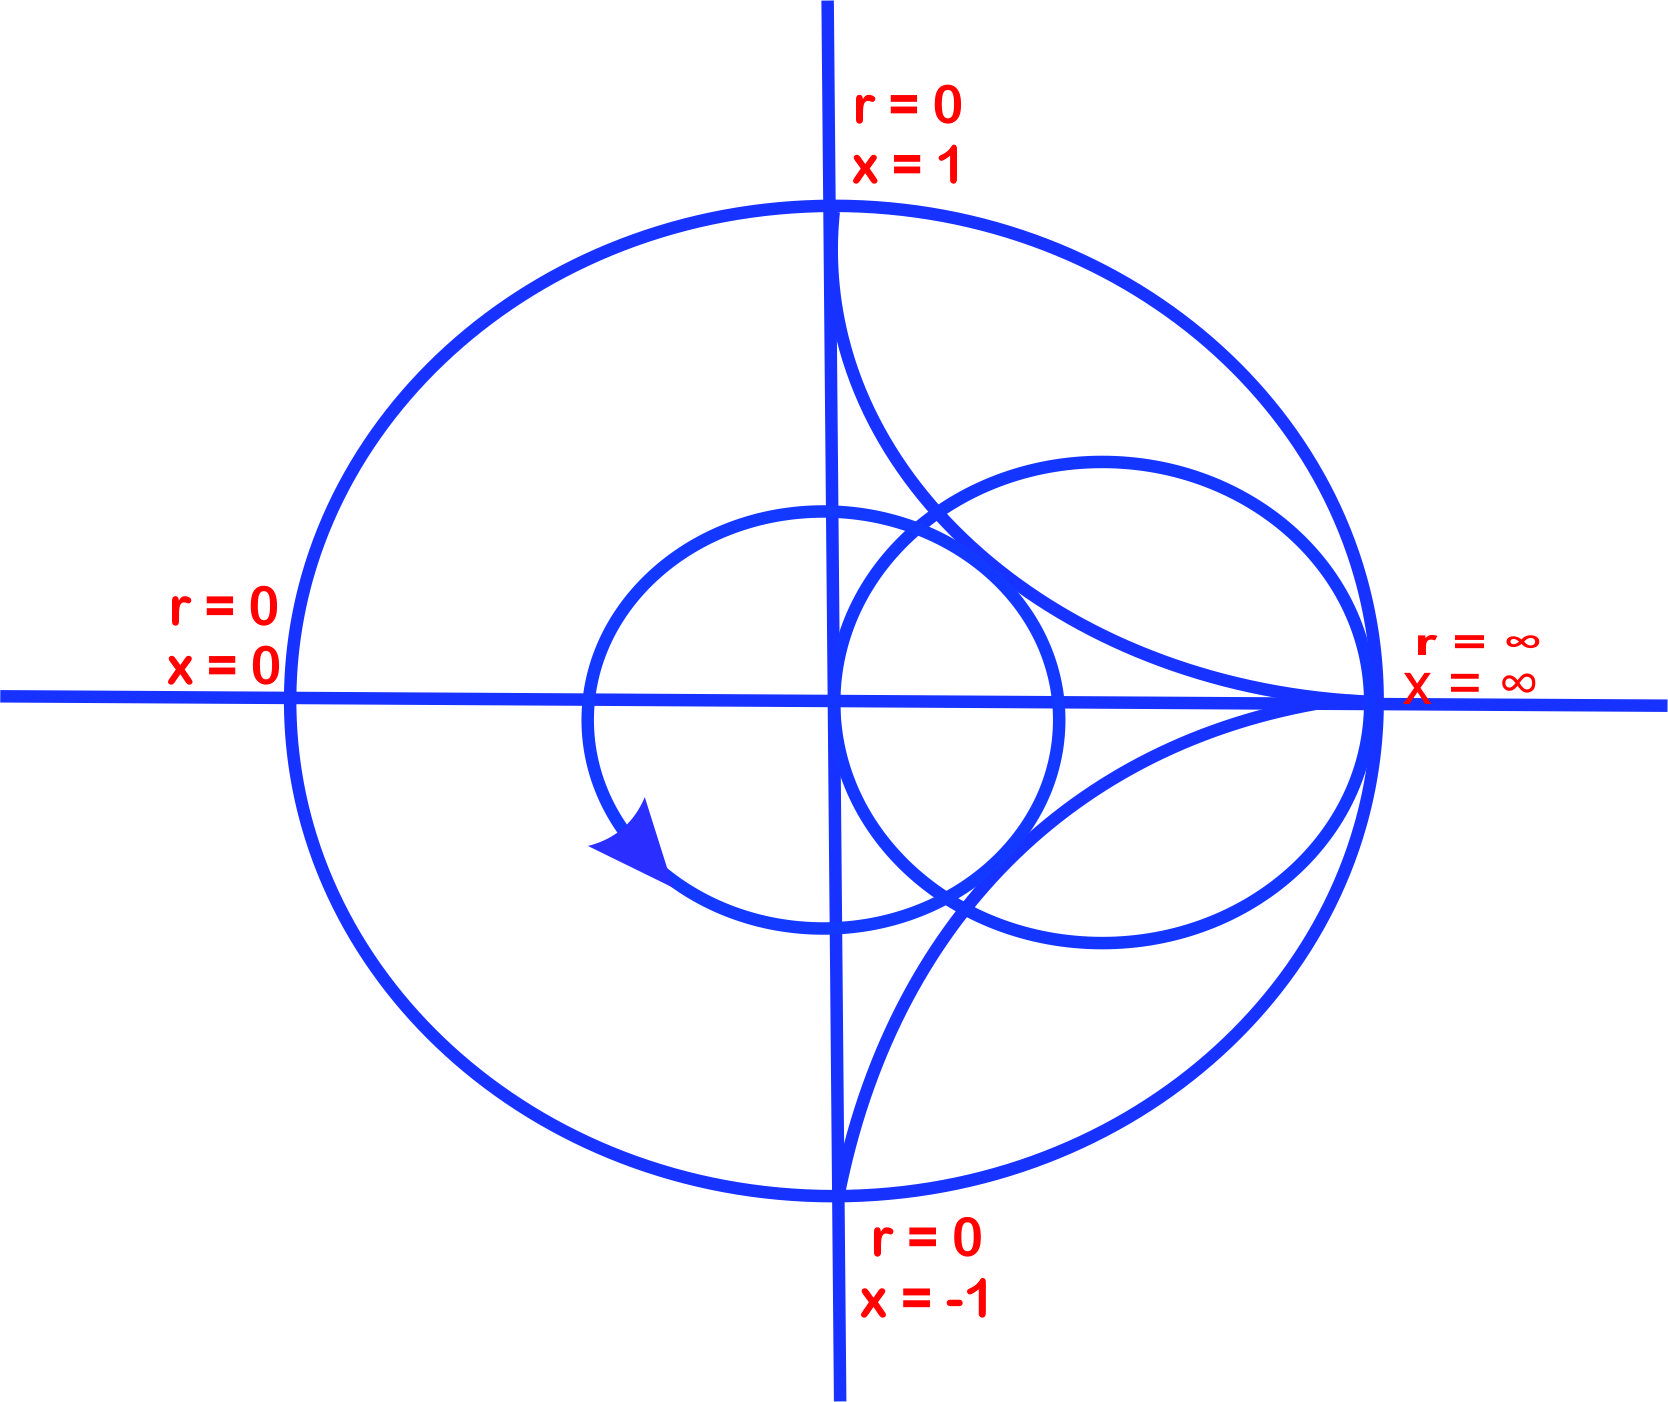
\includegraphics[width=0.5\linewidth]{./graphics/uytrewsxcvbj}
\caption{Points Along the constant r and x Circles}
\label{fig:uytrewsxcvbj}
\end{figure}

\section{Steps in Transmission Line Calculation}
\textbf{Step 1}: If the impedance is not normalized, we normalize all impedances\\
\textbf{Step 2}: Determine all $r$ and $x$ constants from $\overline{Z} = r + jx$ and plot both points to intersect on the smith chart.
As we have seen earlier, the magnitude of the reflection coefficient remains same as the point moves on a circle (
that is, a constant VSWR circle)\\
\textbf{Step 3}: Take a compass and draw a circle passing the point $\overline{Z}_L$ from the origin.\\
NOTE that as we move along the transmission line, the phase angle changes by $2\beta{l}$ in the clockwise direction (from load towards generator).\\
Normally, in a standard smith chart, instead of marking this angle, the distance is marked directly around the smith chart. But how is this done?\\
In one rotation, the angle changes by 2$\pi$, that is, 2$\beta{l}$ = 2$\pi{l}$ = 2(2$\pi/\lambda){l}$ , $l$ =$\lambda/2$ therefore, a full rotation around the smith chart corresponds to a distance of $\lambda/2$ on a constant VSWR circle, then we arrive at the same point.\\\\
The above analysis makes sense since one characteristics of the transmission line is that it's impedance characteristics repeats every $\lambda/2$ and the angle which is now the load angle minus 2$\beta{l}$ can be calibrated in terms of wavelength with a full rotation corresponding to $\lambda/2$ movement. To move from $\overline{Z}_{l}$ by a distance $l_1$, we rotate or move along the circle by an angle of 2$\beta{l}$ clockwise direction (from load towards generator) so $l$ is positive and the angle 2$\beta{l}$ becomes negative. Sense of rotation is very important in doing  all transmission line calculations. If we move in a clockwise direction by a distance of 2$\beta{l}$, we will reach a location $l$ on the transmission line so the intersect point after moving $l$ distance keeps the magnitude of the reflection coefficient. We get a new angle smaller than the previous angle.\\

$\Gamma_{l}$ is what is represented at the point of intersection after moving distance $l$ or angle -2$\beta{l}$. From the new point of  intersection, we find out the constant resistance and reactance circle that passes through $\overline{Z}_{l} = r + jx$ then we multiply by characteristics impedance $Z_o$ to get $\overline{Z}_{l}$ at the new location. Analytically, the impedance transformation requires the calculation of sine and cosine functions that are unusually very complicated. With the help of the smith chart, the impedance transformation is easily achieved.\\\\
One may have a general situation where impedance is given at a particular location and we are told to transform the impedance to another location. Take note, if the new location is to the left of the previous impedance then we do exactly the same thing that has been done as "l" was usually to the left of $Z_{l}$, else we reverse the direction of the angular rotation instead of -2$\beta{l}$, we have $+2\beta{l}$ which is counter-clockwise rotation. Hence, moving towards generator will be clockwise rotation and moving away from generator will be anti-clockwise rotation. The sense of rotation in impedance calculations is extremely important because that tells us whether you are moving towards the generator or away from the generator.Therefore, in all transmission line calculations, the direction of the generator should be given much consideration because that will decide the movement along the transmission line. \\\\
If we replace the impedances by the admittances,and are now interested in only the transformed admittances, then the axis for reflection coefficient comes into picture but every other parameters remains the same like the impedance case until we are required to find the phase of the reflection coefficient and at that point, the positive real axis becomes the one shown below.
\begin{figure}[h]
\centering
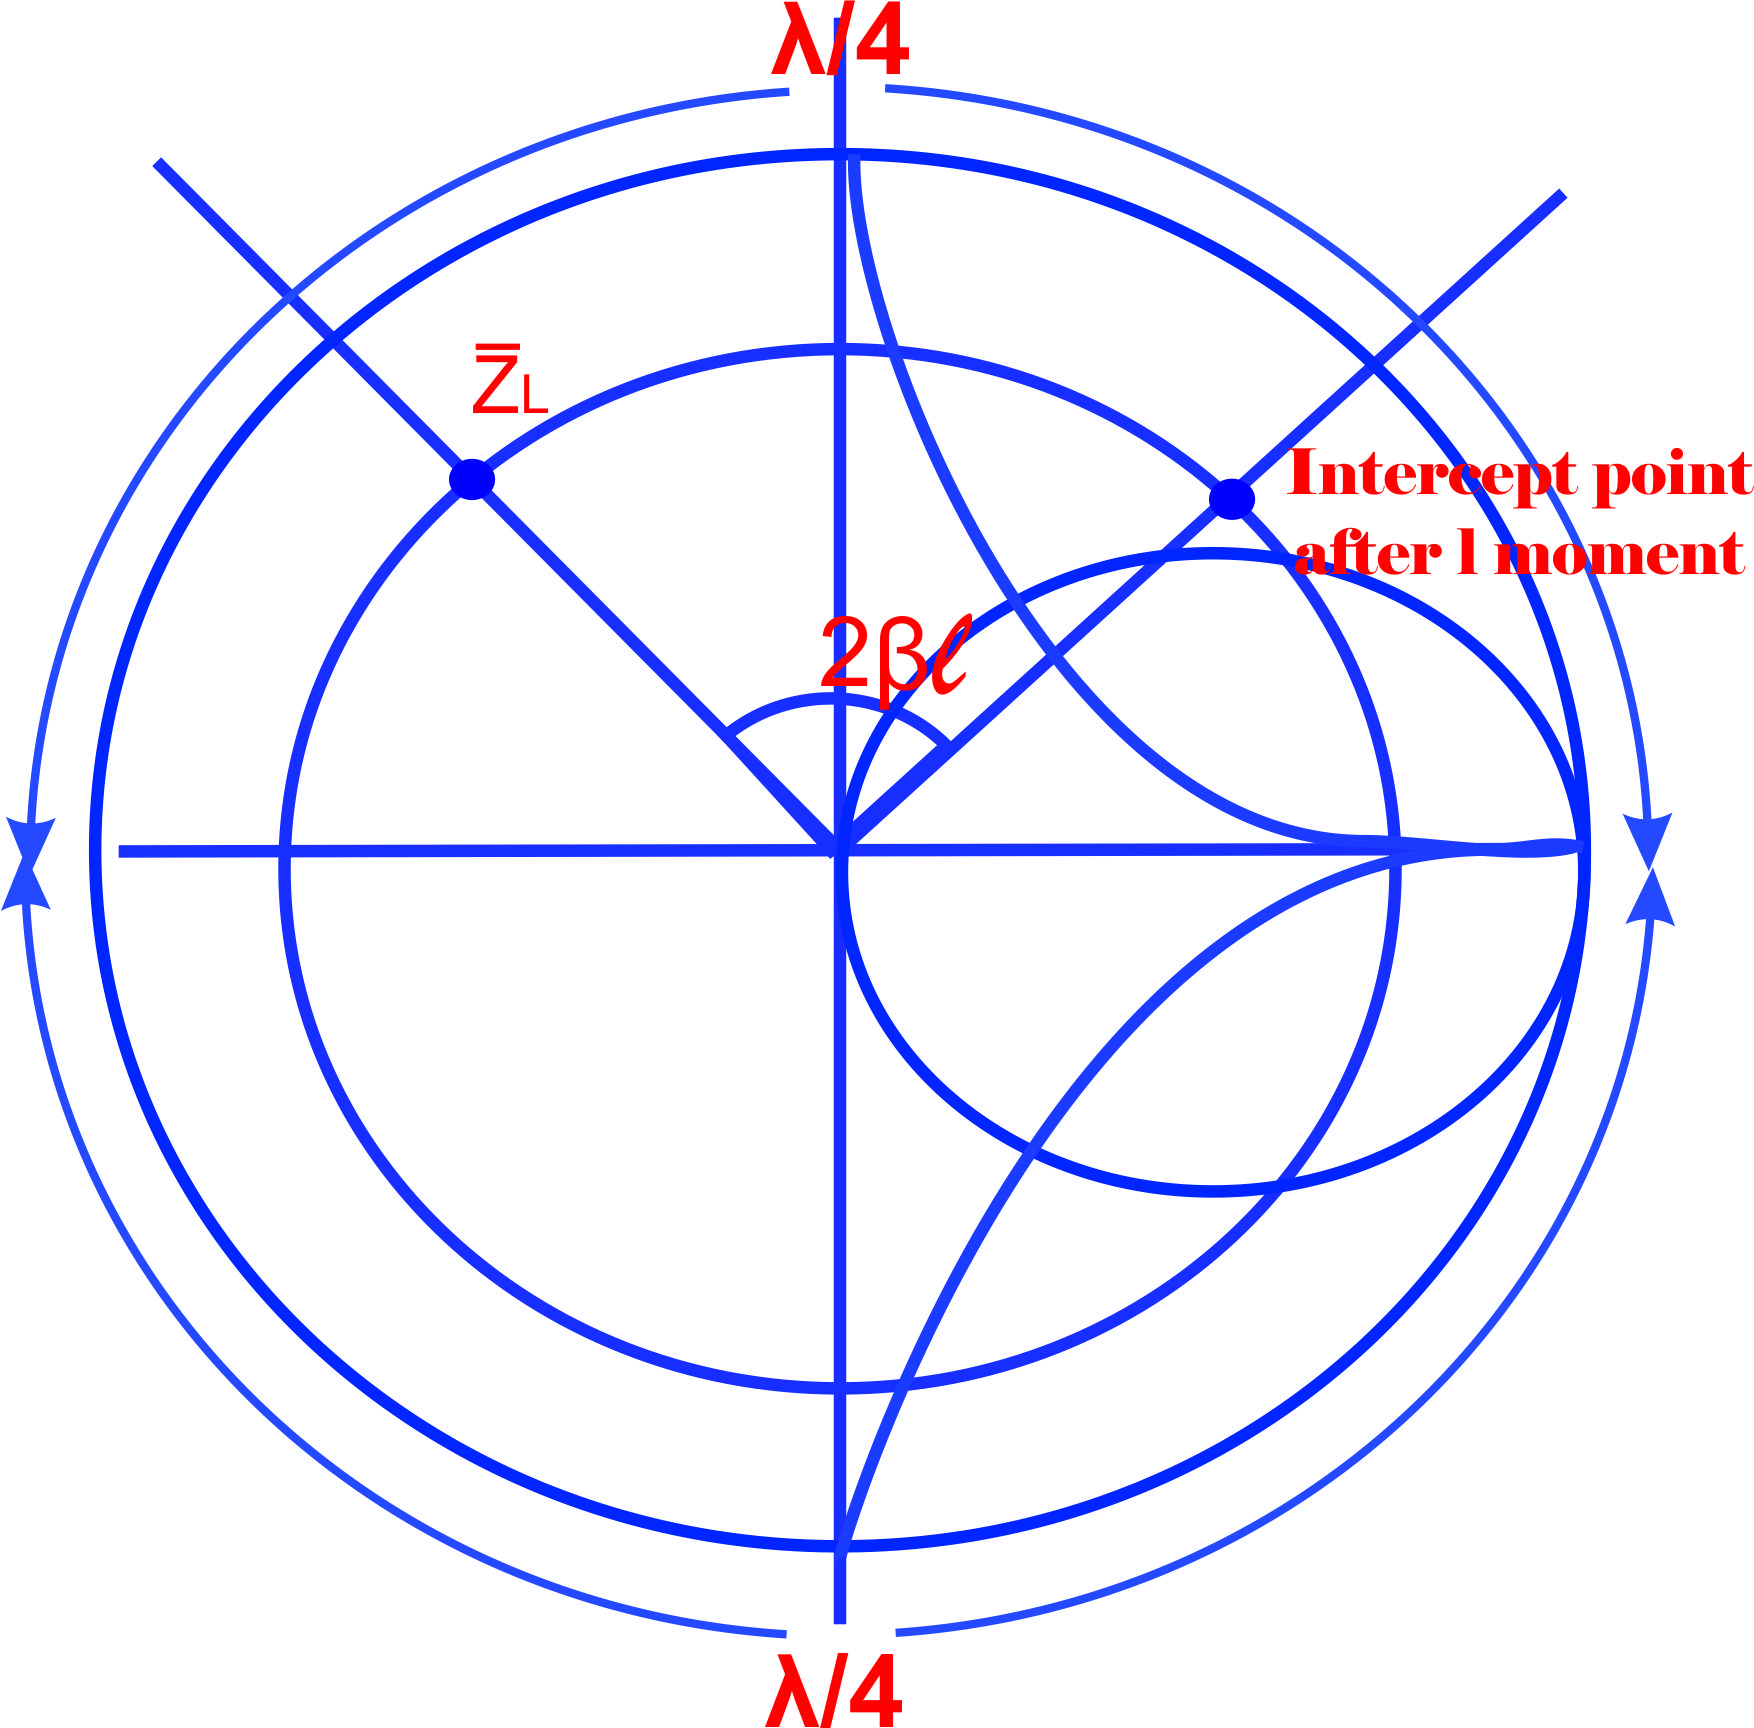
\includegraphics[width=0.5\linewidth]{./graphics/mjhtre}
\caption{Impedance Transformation from Distance L along the Transmssion Line}
\label{fig:mjhtre}
\end{figure}

\subsection*{Procedure:}
\begin{figure}[h]
\centering
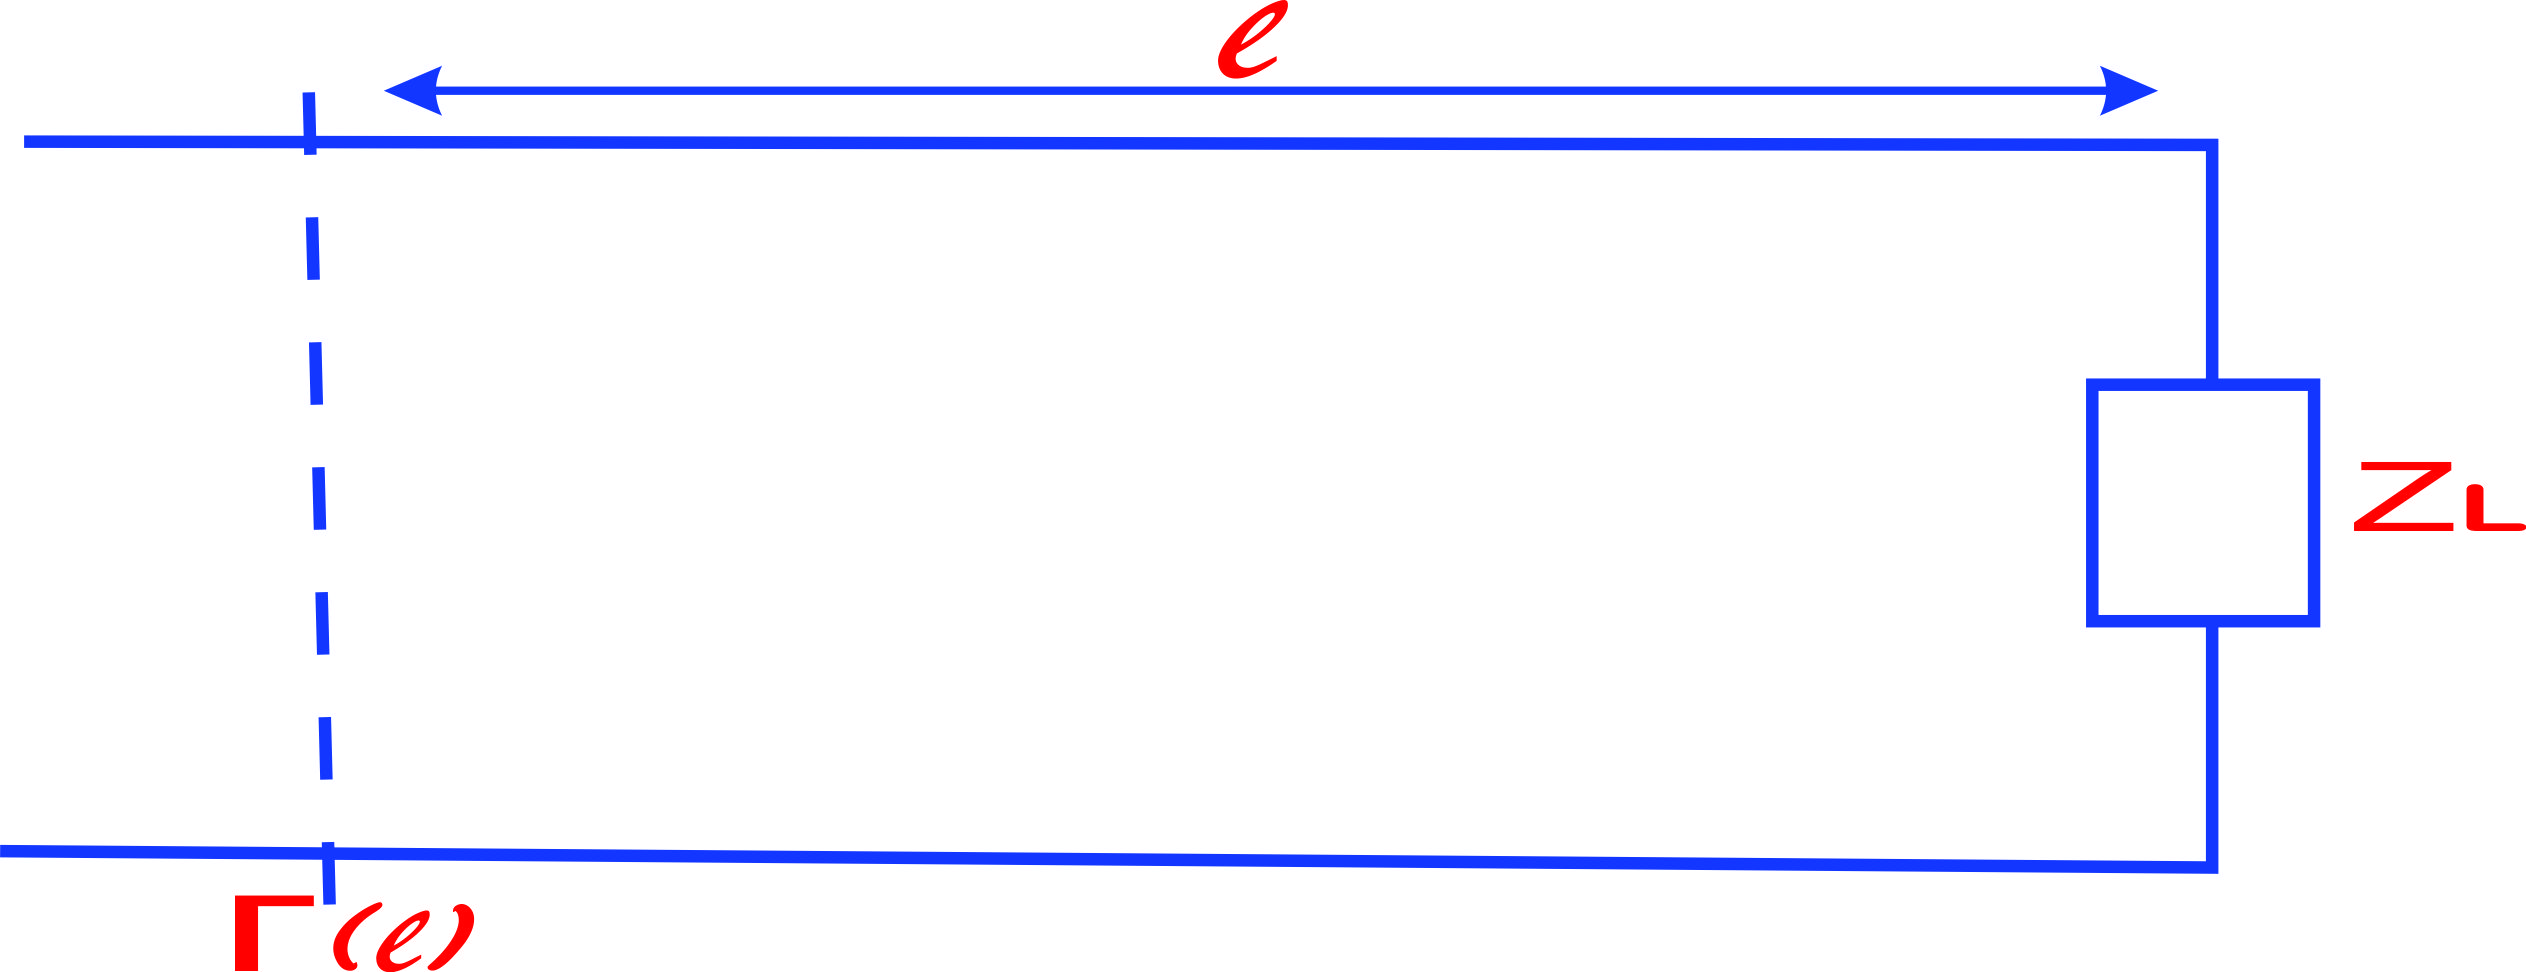
\includegraphics[width=0.7\linewidth]{./graphics/wertuyuk}
\caption{Impedance Transformation by Distance $l$ Along the Transmission Line}
\label{fig:wertuyuk}
\end{figure}
\begin{figure}[h]
\centering
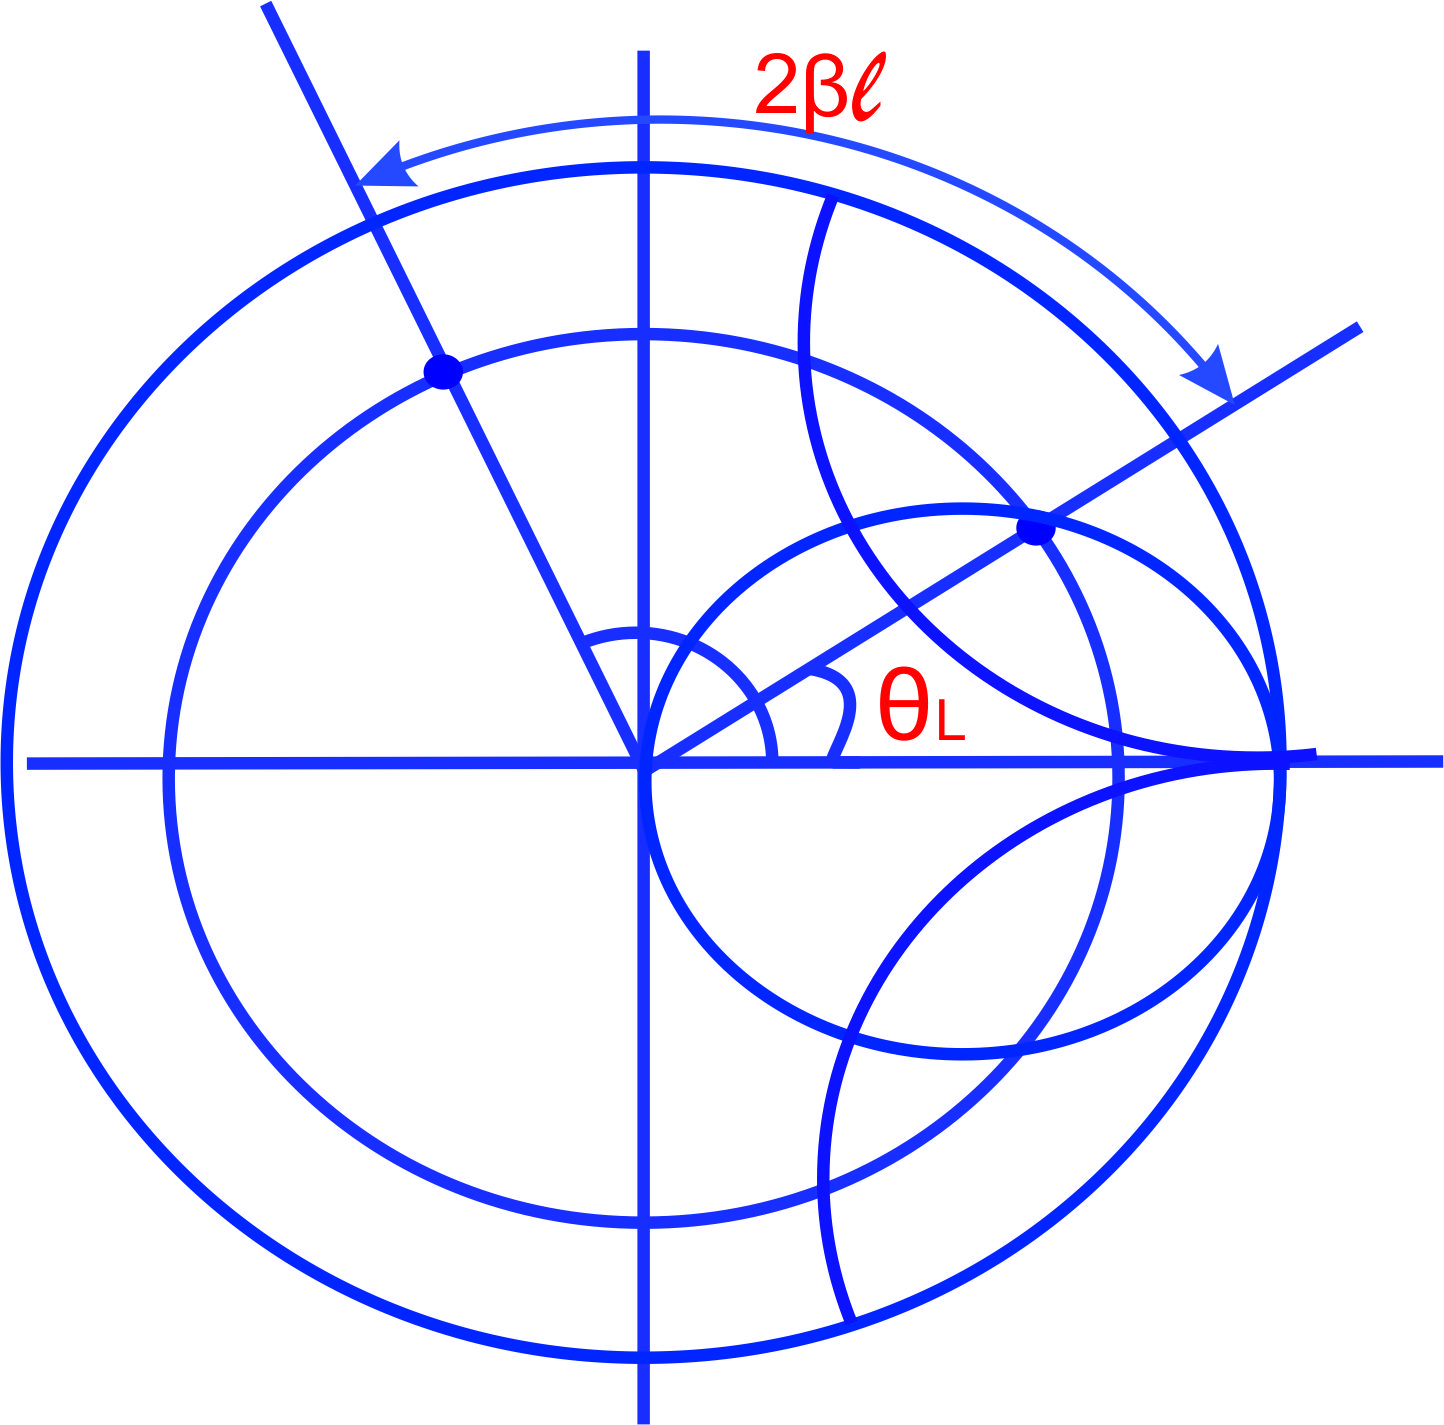
\includegraphics[width=0.5\linewidth]{./graphics/uyhbgjvkclxse}
\caption{New phase Angle after Rotation}
\label{fig:uyhbgjvkclxse}
\end{figure}

Hence, the maximum value of the normalized resistance gives VSWR. Maximum value of resistance in terms of normalized quantity is seen when the VSWR circle intersects the real axis on the right side.The rightmost side corresponds to the impedance which is $R_{max}$ normalized and the reactance for that is zero. Normalized $R_{max}$ is nothing but $\rho$. Similarly, the minimum value which we see on transmission line is $R_{min} = \frac{Z_o}{\rho}$, $\overline{R}_{min} = \frac{1}{\rho}$. The minimum resistance which corresponds to the leftmost intercept on the real axis gives $\frac{1}{\rho}$. Once the load impedance or any other impedance is marked on the smith chart and the constant VSWR circle is drawn, calculation of the VSWR, reflection coefficient and transformed/normalized impedance is very straightforward. It is just a matter of plotting and reading different values on a smith chart.\\\\
Next is to find out the locations of the  minimum and maximum voltage and current on the transmission line. Parameters gotten can be used to determine what kind of loads the transmission line is terminated on by simply looking at the standing wave pattern. A position of a hypothetical load impedance on the smith chart is shown below.
\begin{figure}[h]
\centering
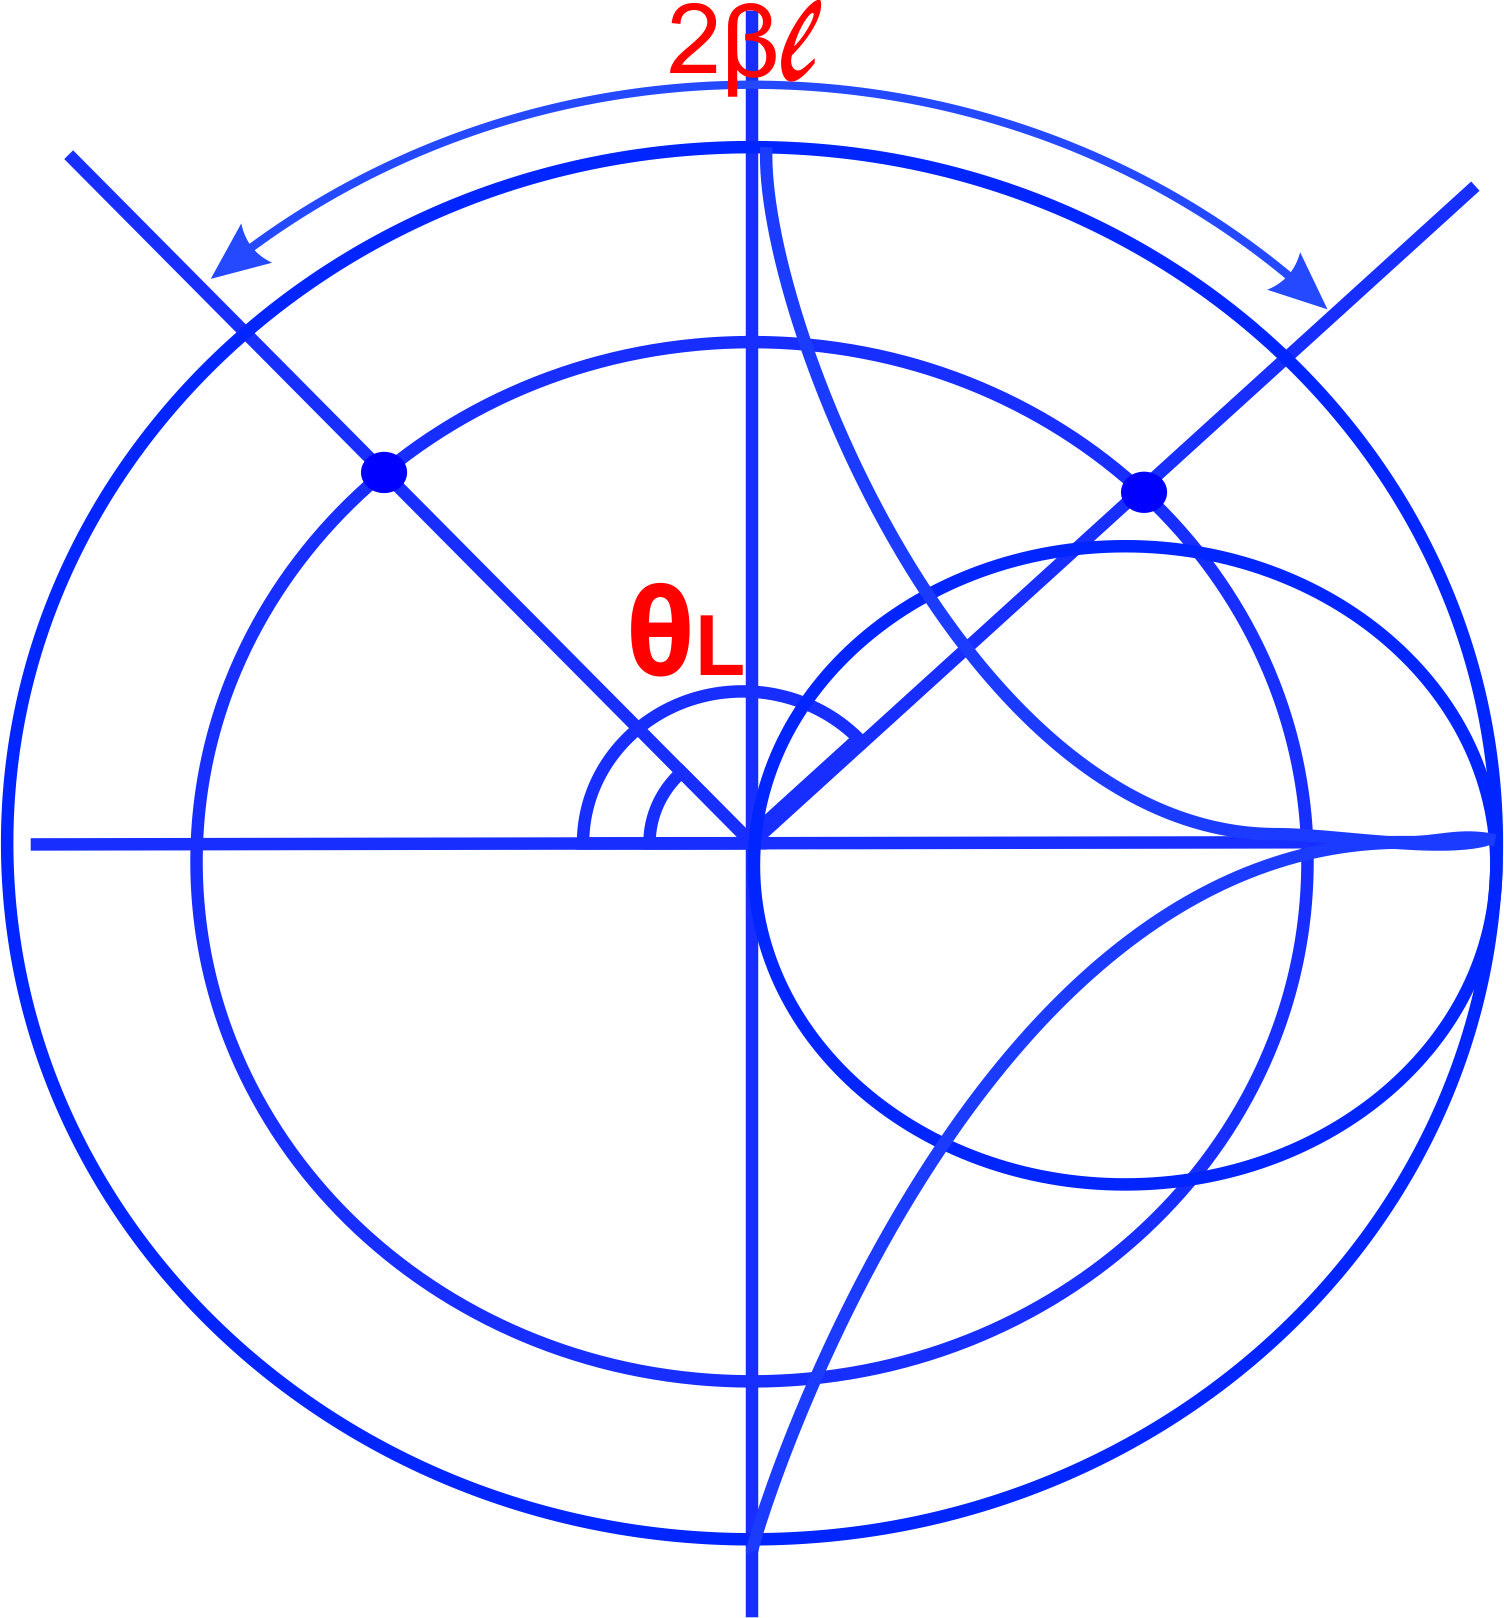
\includegraphics[width=0.4\linewidth]{./graphics/dfyui}
\caption{Change in phase angle at new admittance replacement}
\label{fig:dfyui}
\end{figure}


\section{VSWR on the transmission line}

We want to find out the distance of current or voltage maximum at the load end of the transmission line.
\begin{figure}[h]
\centering
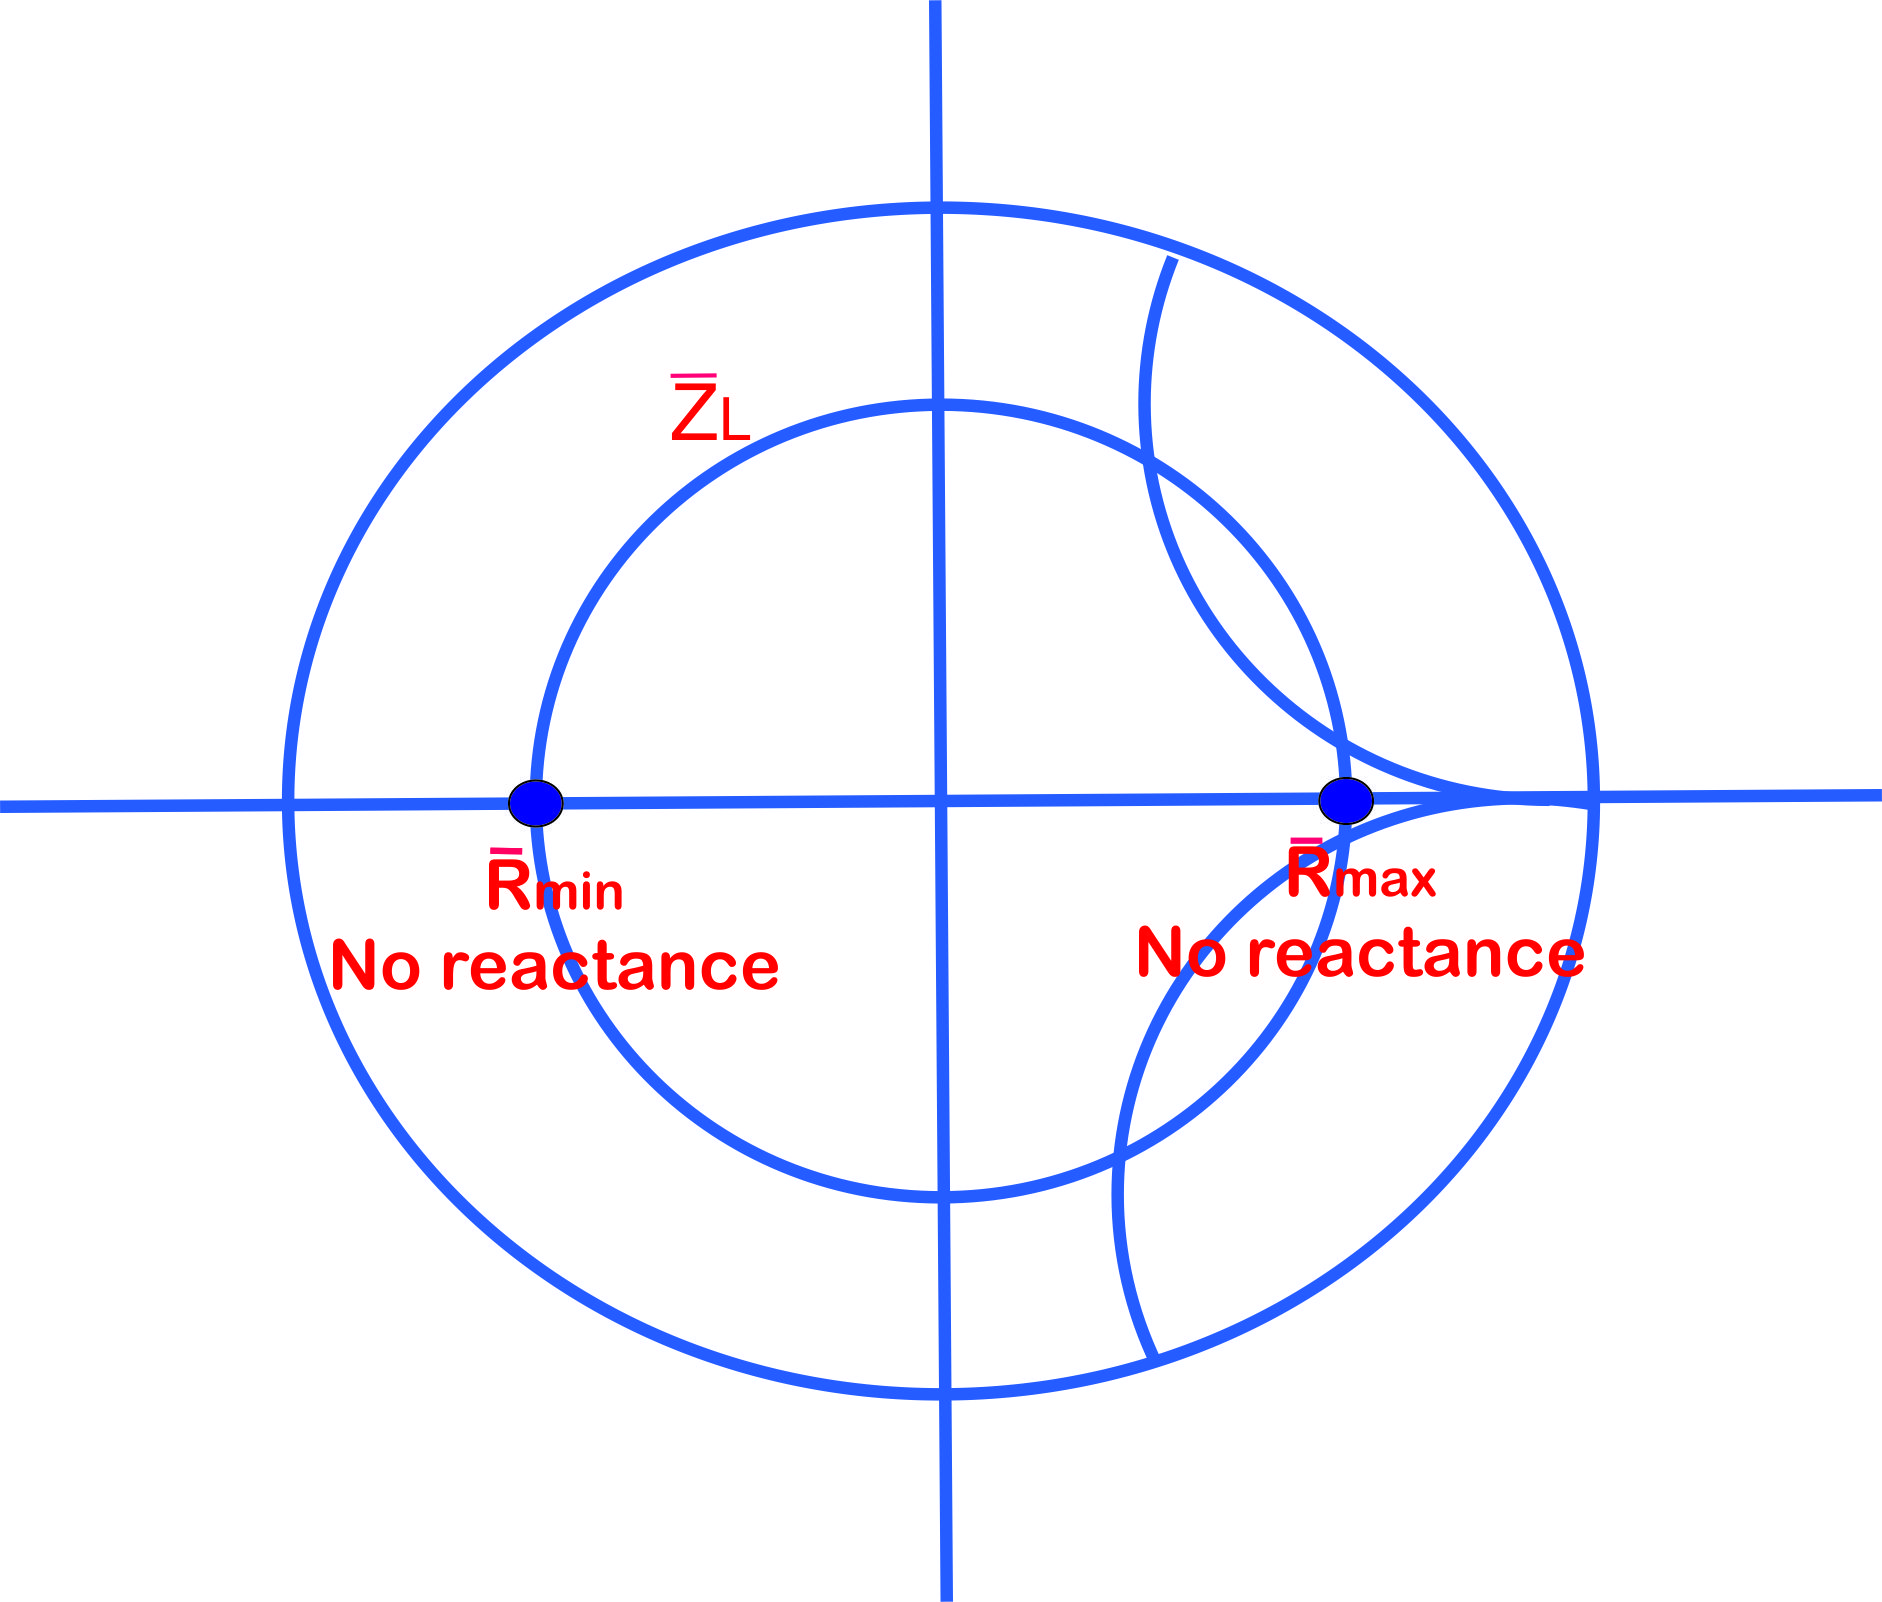
\includegraphics[width=0.7\linewidth]{./graphics/oijhgfdsa}
\caption{Maximum and Minimum Points of Resistance}
\label{fig:oijhgfdsa}
\end{figure}

From our knowledge of transmission line, at point of maximum voltage, we experience minimum current which gives $R_{max}$ then at minimum voltage, we experience maximum current which gives $R_{min}$ hence $R_{max}$ corresponds to $V_{max}$,  $I_{min}$ and  $R_{min}$ corresponds to  $V_{min}$, $I_{max}$.  We want to find out these locations on the load. To move from point $Z_{l}$ to $\bar{R}_{max}$, the clockwise angle covered indicates movement $l$ towards the generator corresponding to $\theta_{max}$ while $\theta_{min}$ corresponds to $180^o$ or $\frac{\lambda}{4}$ distance to get to $R_{min}$ from the $R_{max}$ point.
\begin{figure}[h]
\centering
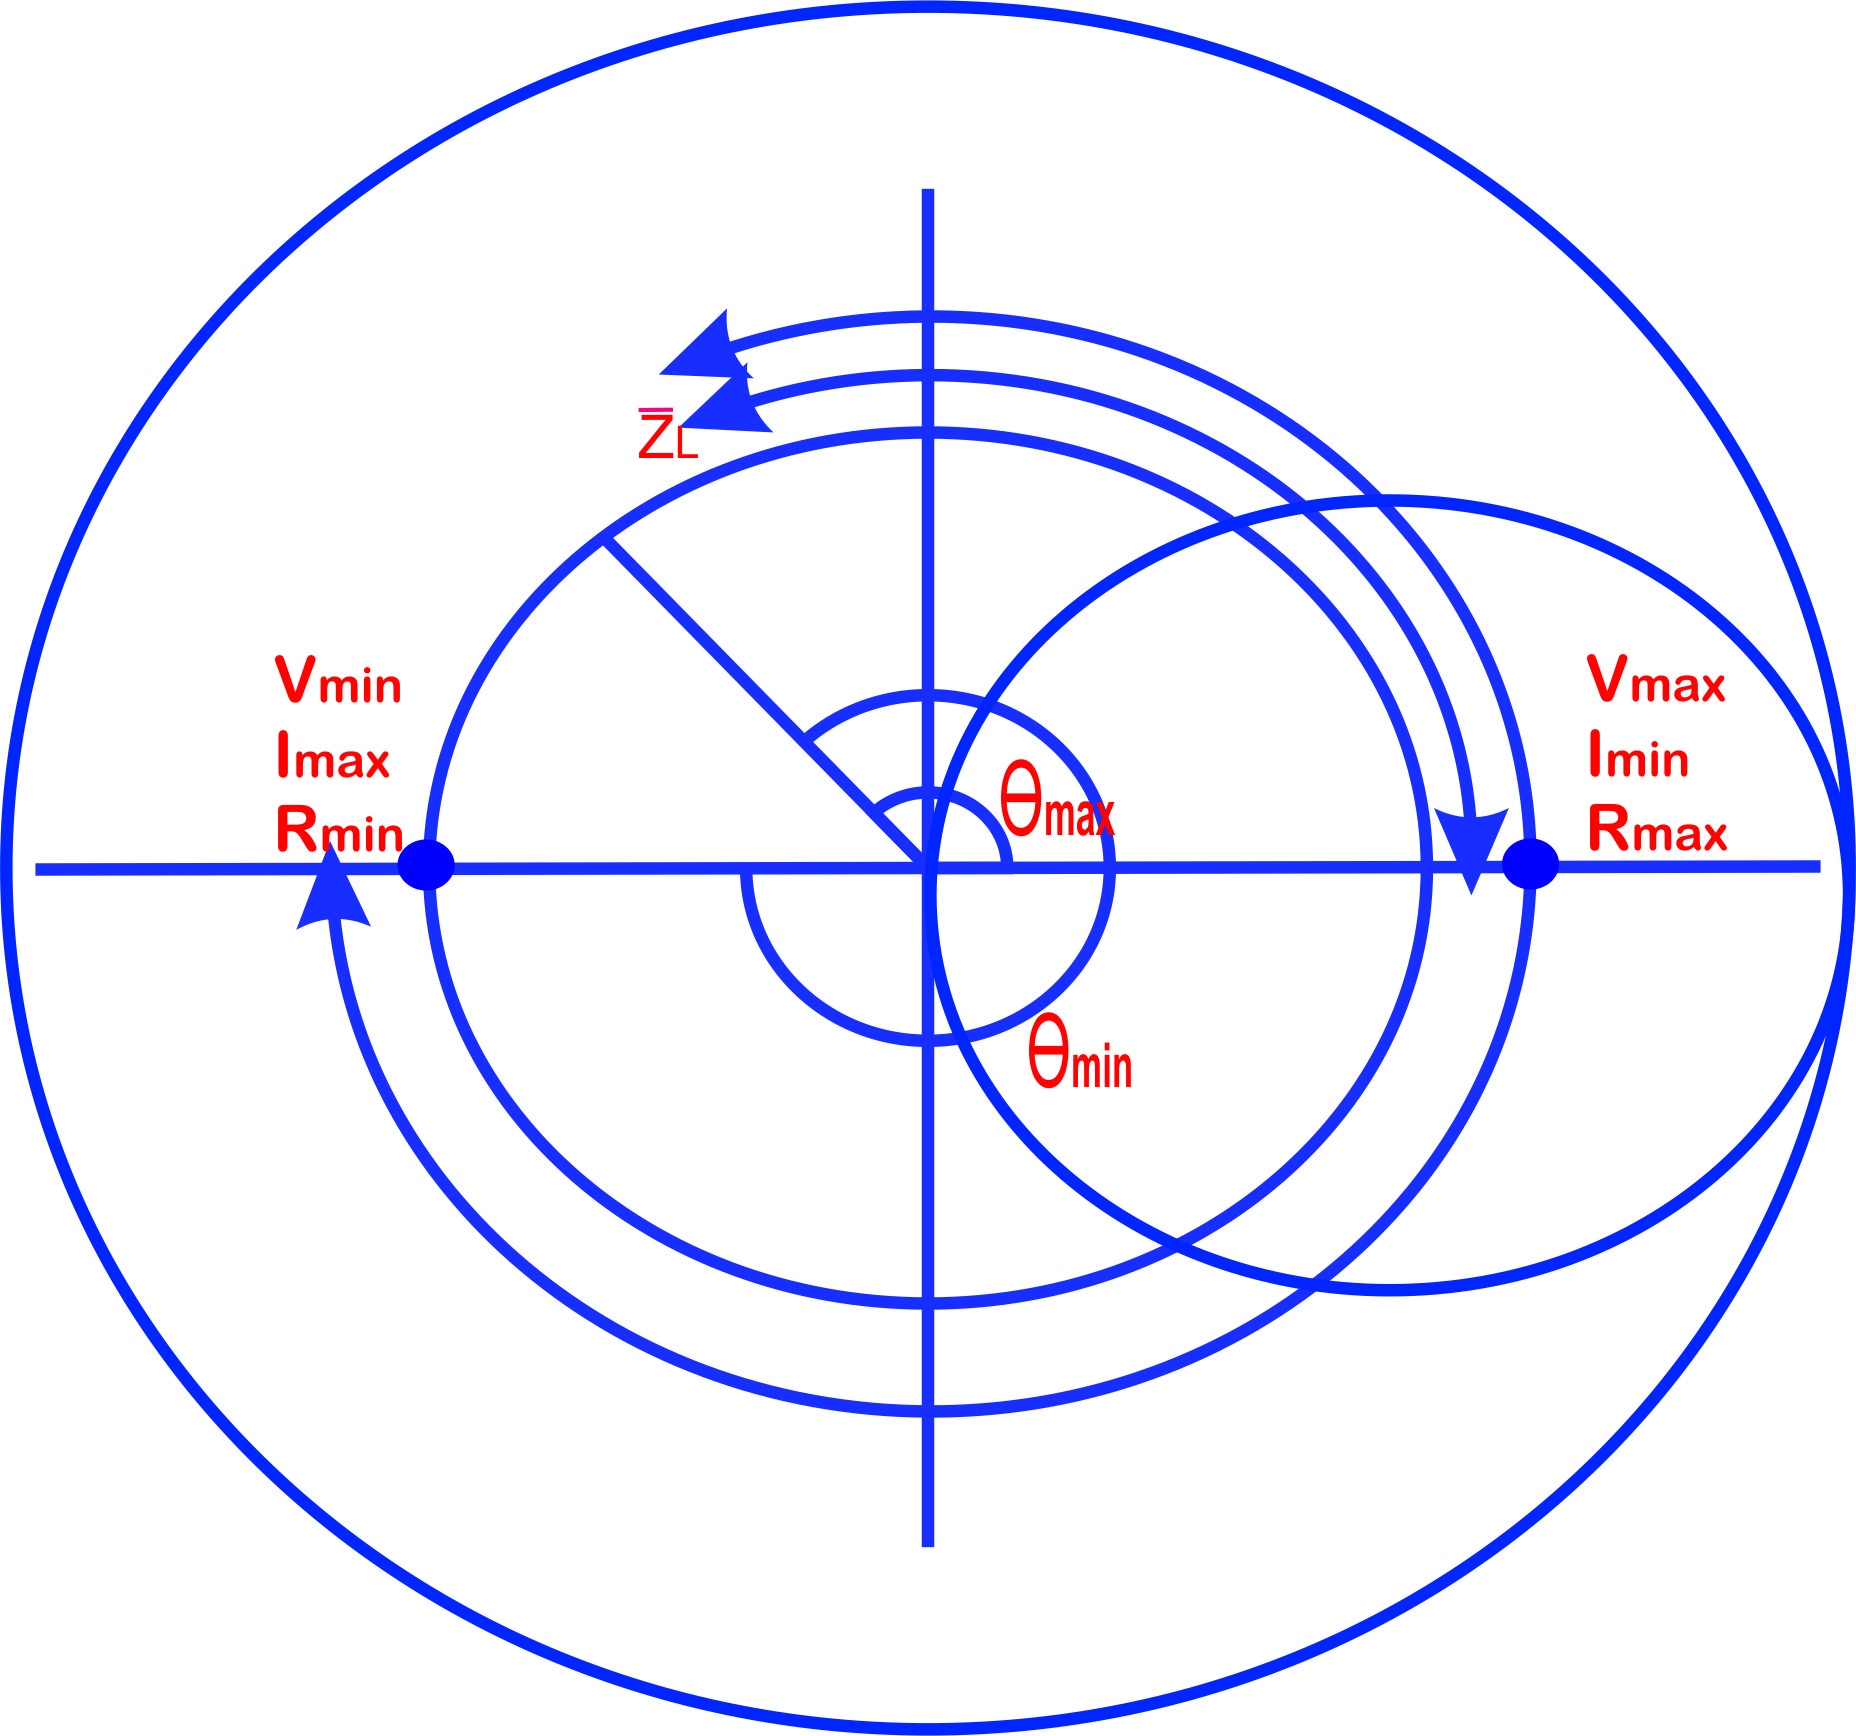
\includegraphics[width=0.6\linewidth]{./graphics/lkjtresx}
\caption{Maximum and Minimum Value of Voltage, Current, and Resistance}
\label{fig:lkjtresx}
\end{figure}

$\frac{\theta_{max}}{2\beta}=l$ gives the distance from the load point $\theta_{max} < 180^o$. From the diagram, $\theta_{min}$ indicates that the angle moved to get to $R_{min}$ is $>270^o but <360^o$. $\theta_{max}$ is therefore the angle moved to get from load to $R_{max}$.
\begin{align}
\frac{\theta_{min}}{2\beta}=\frac{\theta_{max} + \pi}{2\beta} = L
\end{align}
To get to $R_{min}$ position; $\theta_{min} = \frac{\theta_{max}}{2\beta} + \frac{\lambda}{4}.$ 